\chapter{Diseño}
\label{cap:capitulo4}


\vspace{1cm}
El principal objetivo de este TFG es desarrollar un sistema autónomo de navegación para un dron en entornos de simulación. Este dron debe ser capaz de desenvolverse
por carreteras urbanas con un comportamiento reactivo y seguro. 
Para lograr este objetivo, se implementa la infraestructura de comunicaciones entre el entorno de simulación y las diversas 
plataformas de desarrollo. Esta infraestructura permite la transferencia de datos en tiempo real y la integración de diferentes módulos del sistema, garantizando 
una comunicación fluida y eficiente.

Posteriormente, se desarolla el sistema perceptivo mediante inteligencia artificial junto con el desarrollo de comportamientos autónomos tradicionales utilizados en diferentes robots, como el seguimiento de carriles. Entre los métodos utilizados, se incluye 
el control clásico basados en controladores y métodos de control avanzados basados en aprendizaje por refuerzo, con el fin de que el dron aprenda y se 
adapte a diferentes escenarios urbanos. 

Una vez desarrollados estos comportamientos, se procede a realizar una evaluación exhaustiva de los resultados obtenidos, 
recopilando diferentes métricas para determinar la efectividad de cada enfoque y adapatabilidad del dron. 
Finalmente, se analizan los resultados y se realiza una comparativa, destacando las ventajas y limitaciones, proporcionando así una visión global del desesempeño del sistema autónomo 
de navegación del dron utilizando aplicaciones de entornos urbanos. 


\section{Arquitectura}
\label{sec:Arquitectura}

La arquitectura propuesta para este trabajo como se muestra en la figura \ref{fig:infraestructura} consta de dos componentes principales 
comunicados entre sí: El entorno de simulación  y las plataformas de desarrollo. En estas plataformas se desarrollan tanto el sistema perceptivo 
como el de control, permitiendo una integración robusta y eficiente de las funcionalidades del dron en un entorno controlado y seguro. Estos componentes 
están distribuidos en dos ordenadores distintos, denonimados PC1 y PC2. 

Por un lado, el primer componente está compuesto por el entorno de simulación Airsim, ejecutado en el PC1. Incluye la configuración de sensores y actuadores necesarios 
para la navegación del dron. La comunicación entre este componente y el segundo componente (PC2), se realiza a través de dos interfaces principales: 

\begin{enumerate}
  \item \textbf{ROS Wrapper Airsim Node}: Este componente actúa como una interfaz que facilita la integración de Airsim con el middleware ROS. A través del ROS Wrapper Airsim, 
  se recogen tres tipos de salidas: 
    \begin{enumerate}
      \item \textbf{Imágenes RGB}: Capturadas por las cámaras a bordo del dron, estas imágenes son fundamentales para el sistema perceptivo, permitiendo la detección y el 
      seguimiento del carril.
      \item \textbf{Altura}: Obtenida a través del sensor Lidar, esta medida es esencial para conocer la altura a la que vuela el dron durante su navegación. 
      \item \textbf{Localización}: Proporcionada por el GPS, esta información permite conocer la posición del dron en el entorno simulado. 
    \end{enumerate}

  \item \textbf{Client Airsim}: Este componente permite el control del dron, gestionando las velocidades lineales y angulares necesarias para su navegación. 
\end{enumerate}

Dentro de PC2, se encuentra un componente denominado Nodo ROS que encapsula el sistema perceptivo y el seguimiento de carril, actuando como el nucleo de 
procesamiento. Este nodo recibe y procesa las entradas de los sensores (imágenes RGB, altura y localización), y como salida genera velocidades lineales y angulares, teniendo
como submódulos: 

\begin{enumerate}
  \item \textbf{Percepción}: Utilizando las imágenes RGB proporcionadas por ROS Wrapper Airsim a través del sensor de la cámara del dron, este sistema procesa la información
  visual para detectar el carril en el que debe navegar el dron. La detección del carril es fundamental para la ejecución del comportamiento sigue-carril, que guía al dron 
  a lo largo del carril deseado. 
  \item \textbf{Sigue-Carril}: Este comportamiento se encarga de seguir una trayectoria predefinida basada en la detección del carril. Dentro de este componente, se 
  utiliza dos enfoques diferentes: 
  \begin{enumerate}
    \item \textbf{PID}: Un enfoque clásico de control que ajusta las velocidades angulares y teniendo una velocidad lineal constante del dron en función de las desviaciones
    del carril detectado.
    \item \textbf{Aprendizaje por Refuerzo}: Un enfoque más avanzado que utiliza técnicas de aprendizaje automático para optimizar el comportamiento del dron. Este método 
    permite al dron aprender de su entorno en diferentes condiciones. 
  \end{enumerate}

  Ambos enfoques de control generan comandos de velocidades lineales y angulares que son enviados al Client Airsim. Este, a su vez, traduce estos comandos en acciones físicas 
  en el entorno simulado, permitiendo el movimiento controlado y preciso del dron. 
\end{enumerate}

\begin{figure} [H]
    \begin{center}
      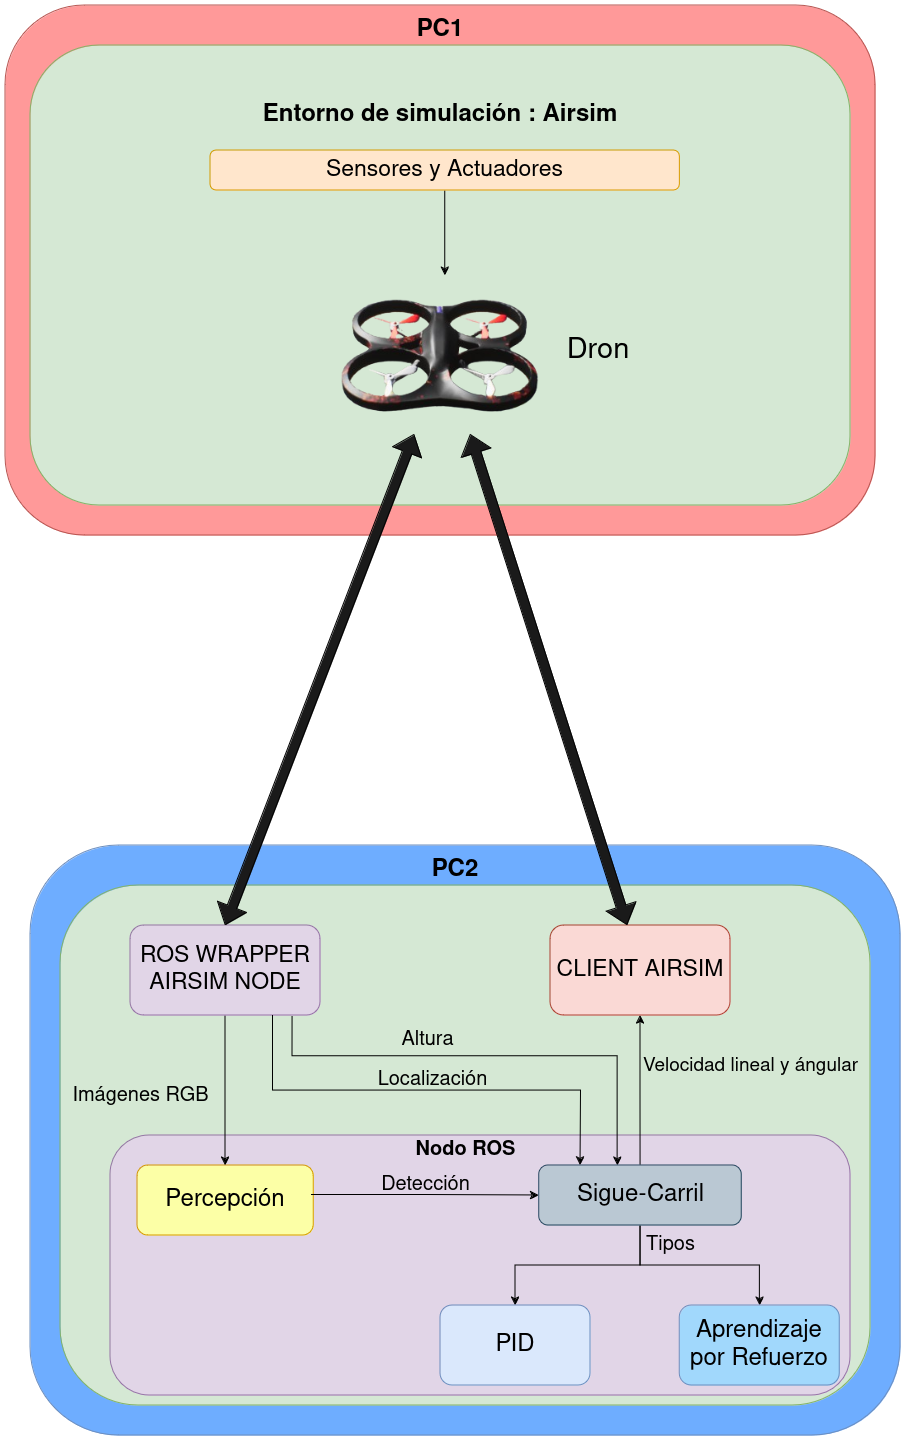
\includegraphics[scale=0.30]{figs/Diseño/Comunicaciones/diagrama_arquitectura.png}
    \end{center}
    \caption{Arquitectura general del desarrollo en este TFG}
    \label{fig:infraestructura}
  \end{figure}\

\section{Distribución de equipos}
\label{distribución}
En el desarrollo de este TFG, hemos decidido adoptar un enfoque distribuido. El entorno de simulación, compuesto por Airsim y UnrealEngine, se ejecuta en un ordenador con un sistema 
operativo Windows 10 y una GPU Nvidia RTX 2070 Super. Por otra parte, las plataformas de desarrollo, que incluyen ROS, AirSim ROS Wrapper Node y Client Airsim se ejecutan en un ordenador secundario 
con un sistema operativo Ubuntu 20.04 y una GPU Nvidia RTX 2070.

Esta propuesta se tomó con la iniciativa de no encapsular en un único componente el entorno de simulación y las plataformas de desarrollo. Inicialmente, todo el sistema 
seguía una configuración centrazalida en un solo equipo con Ubuntu 20.04, generando cuellos de botella y limitando al rendimiento del sistema. Para solventar estos problemas, 
se diseñó una infraestructura distribuida entre dos ordenadores distintos, diviendo así la carga de trabajo entre los dos sistemas. Por un lado, el primer ordenador se
ejecuta el entorno de simulación Airsim mientras que en el segundo ordenador se manejan las plataformas de desarrollo. \newline

Al principio del desarrollo de esta distribución de equipos, se utilizó una comunicación con PX4 y Mavros, siguiendo la documentación oficial\footnote{\url{https://docs.px4.io/main/en/simulation/}} 
junto con el entorno de simulación Airsim. Sin embargo, se decidió cambiar por una nueva configuración que emplea ROS Wrapper Airsim Node y Client Airsim, ya que 
la comunicación original añadía una capa adicional produciendo bajos rendimientos que afectaba a la sincronización con el simulador. 

En resumen, el sistema de comunicaciones se compone de dos ordenadores interconectados en la misma red. El diagrama 
de comunicaciones ilustrado en la figura \ref{fig:diagramadeAirsim}, muestra esta implementación distribuida en diferentes ordenadores. Cada ordenador asume roles distintos: 
El primer ordenador ejecuta el entorno de simulación en cambio el segundo ordenador, gestiona las plataformas de desarrollo en donde se implementan los algoritmos 
de percepción y seguimiento de carril. Ambos ordenadores se comunican a través de un router teniendo cada uno una dirección IP distinta. 

\begin{figure} [H]
  \begin{center}
    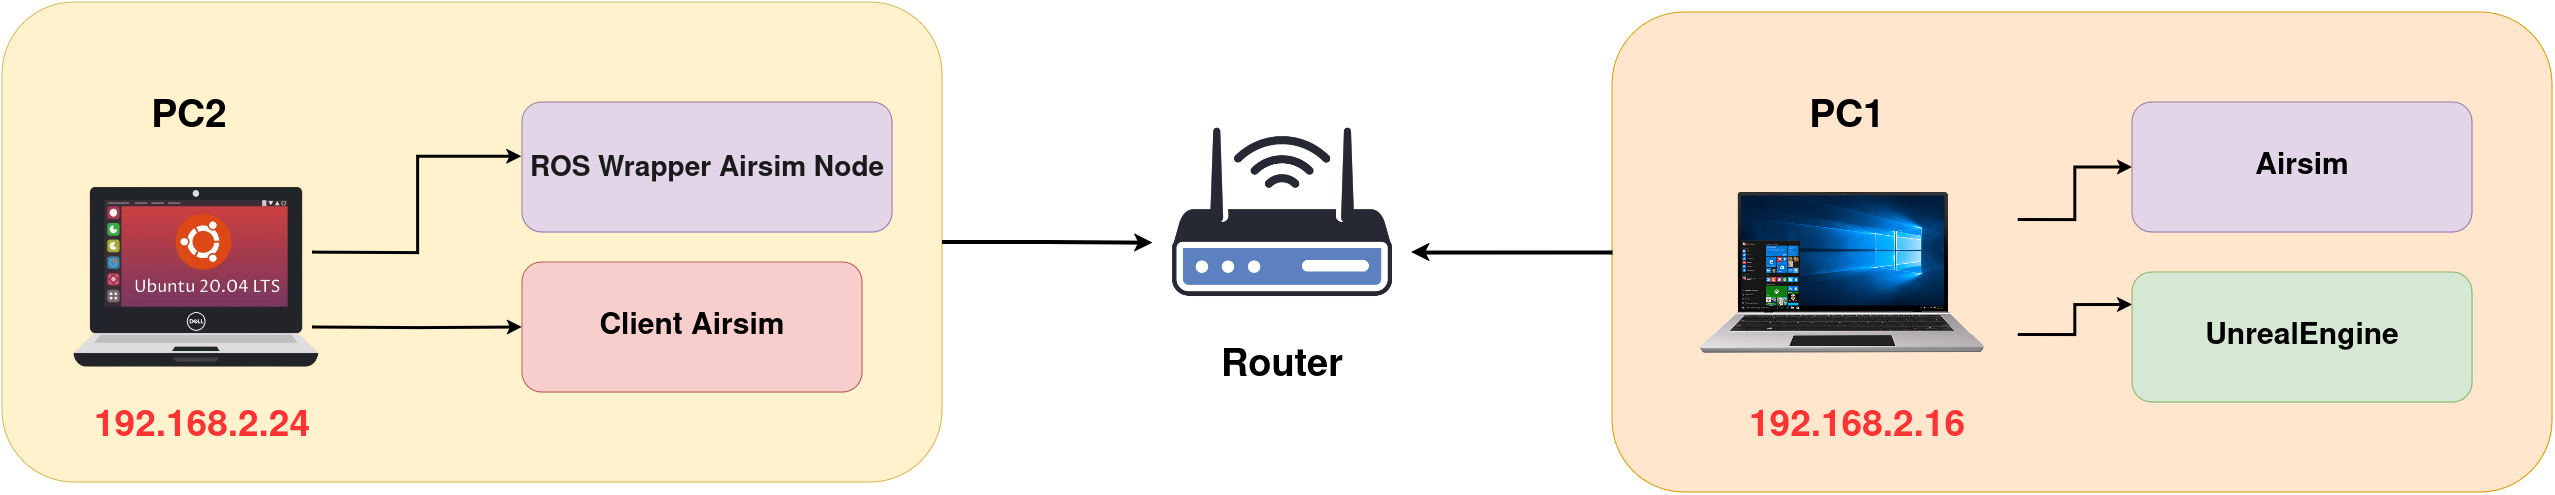
\includegraphics[scale=0.18]{figs/Diseño/Comunicaciones/comunicaciones.png}
  \end{center}
  \caption{Diagrama de comunicaciones}
  \label{fig:diagramadeAirsim}
\end{figure}\

\subsection{Preparación del entorno de simulación}
\label{sec:Preparación_entorno}

Como mencionamos en la sección \ref{sec:Airsim}, utilizamos como simulador Airsim junto con el motor UnRealEngine. Para construir el entorno de simulación, primero
necesitamos instalar UnrealEngine. Para ello, seguimos las instrucciones marcadas por la página oficial de Epic Games\footnote{\url{https://www.unrealengine.com/en-US/download}}, 
utilizando la versión 4.27.2.

Una vez que UnrealEngine esté instalado, procedemos a configurar el entorno de simulación mediante el archivo settings.json. Por defecto, al ejecutar Airsim 
por primera vez, el simulador crea este archivo automáticamente dentro de una carpeta denoninada Airsim en la carpeta Documentos en Windows. Esto 
resulta conveniente, ya que podemos modificar este archivo según nuestras necesidades. 


\subsubsection{Configuración del dron y del entorno}
\label{subsec:Configuración del dron y del entorno}

En primer lugar se utiliza el entorno de simulación Coastline de entre los diferentes entornos que nos ofrece Airsim para Windows. Al descargar esta carpeta, 
se obtiene un fichero ejecutable para abrir el entorno con Airsim, junto con carpetas de modelos de simulación como las carreteras, montañas y vegetación. Dentro de estas carpetas, se eliminan dichos componentes 
de simulación que pueden dificultar al sistema perceptivo, como plantas y señales de tráfico que se ubican en las carreteras, facilitando así la percepción del entorno 
y haciéndolo más manejable. En la figura \ref{fig:CoastlineModificado} se muestra marcado en color rojo, los componentes eliminados del entorno para facilitar al sistema 
perceptivo.

\begin{figure} [H]
  \begin{center}
    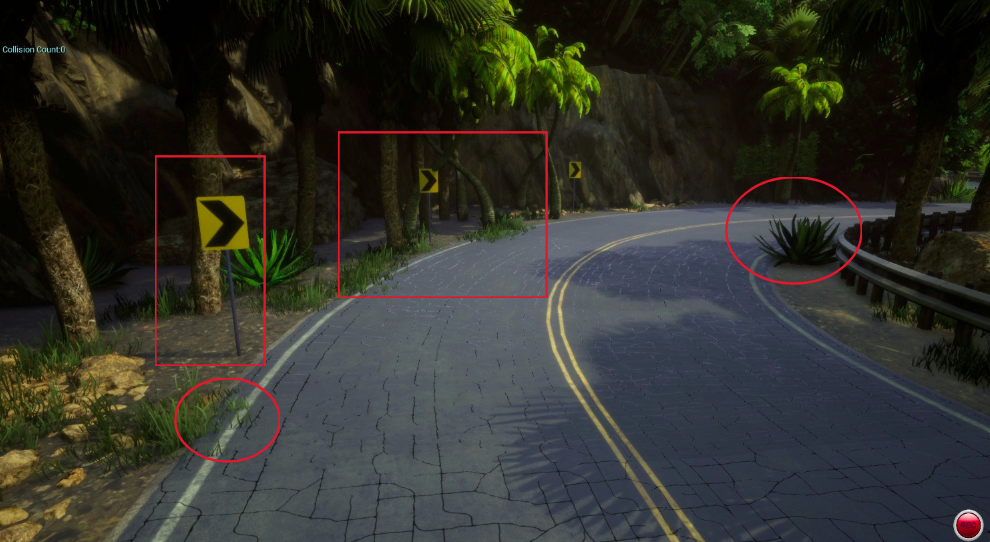
\includegraphics[scale=0.4]{figs/Diseño/coastline3.png}
  \end{center}
  \caption{Visualización del entorno original ilustrando los objetos que dificultan al sistema perceptivo}
  \label{fig:CoastlineModificado}
\end{figure}\

Cuando el fichero settings.json este creado, ya podemos equipar al dron con características como qué sensores va a utilizar, 
el tipo de vehículo, el tipo de simulación, la comunicación y más. Como se muestra en el código \ref{cod:settings}, se definen como sensores el Lidar para saber a que altura
esta volando el dron respecto al suelo, el GPS para conocer la localización que tiene el dron en el entorno y la cámara con imagenes
RGB. Cada sensor debe llevar su propia configuración, siguiendo sus propios parámetros que dicta la guía oficial de Airsim\footnote{\url{https://microsoft.github.io/AirSim/sensors/}}
. La cámara tiene una peculiaridad de que se configura siendo otro sensor a parte de la lista de sensores de Airsim, consta de varios parámetros que se tienen que configurar como 
el tamaño de la imagen, el uso de ROS, los FPS de la imagen transmitida, la posición, etc. 
Los actuadores no es necesario tener ninguna configuración respecto a ellos. 

\begin{figure}[H]
  \centering
  \begin{multicols}{2}
    \begin{lstlisting}[language=json,basicstyle=\tiny,numbers=none]
{
  "SettingsVersion":1.2,
  "SimMode":"Multirotor",
  "ClockType":"SteppableClock",
  "Vehicles":{
     "Drone":{
        "VehicleType":"SimpleFlight",
        "ControlIp":"remote",
        "LocalHostIp":"192.168.2.16",
        "Sensors":{
           "LidarCustom":{
              "SensorType":6,
              "Enabled":true,
              "Range":10,
              "NumberOfChannels":16,
              "RotationsPerSecond":10,
              "PointsPerSecond":10000,
              "X":0,
              "Y":0,
              "Z":-1,
              "DrawDebugPoints":false,
              "DataFrame":"SensorLocalFrame"
           },
           "Gps":{
              "SensorType":3,
              "Enabled":true,
              "EphTimeConstant":0.9,
              "EpvTimeConstant":0.9,
              "EphInitial":25,
              "EpvInitial":25,
              "EphFinal":0.1,
              "EpvFinal":0.1,
              "EphMin3d":3,
              "EphMin2d":4,
              "UpdateLatency":0.2,
              "UpdateFrequency":50,
              "StartupDelay":1
           }
        }
     }
  }
}
    \end{lstlisting}
    \columnbreak
    \begin{lstlisting}[language=json,basicstyle=\tiny,numbers=none]
{
   "Cameras":{
     "front_center_custom":{
        "CaptureSettings":[
           {
              "PublishToRos":1,
              "ImageType":0,
              "Width":620,
              "Height":620,
              "FOV_Degrees":90,
              "ImageRate_FPS":30,
              "TargetGamma":1.5,
              "AutoExposure":true,
              "MotionBlur":false,
              "PostProcess":true
           }
        ],
        "X":0.50,
        "Y":0,
        "Z":0.10,
        "Pitch":0,
        "Roll":0,
        "Yaw": 0
     }
   },
   "X": 22.474933624267578,
   "Y": -25.63629913330078,
   "Z":  0,
   "Pitch": 0,
   "Roll": 0,
   "Yaw":  30
}
    \end{lstlisting}
  \end{multicols}
  \caption[Configuración del dron mediante el fichero settings.json]{Configuración del dron mediante el fichero settings.json}
  \label{cod:settings}
\end{figure}

Si no se define la posición inicial del dron como aparece en la última parte del fichero settings.json, por defecto el propio simulador te establece el vehículo en el punto que decida Airsim. 



  \subsubsection{Instalación de las herramientas de desarrollo}
  \label{subsec:Instalación de las herramientas de desarrollo}
  La instalación de las herramientas de desarrollo como se comentó en la sección de \ref{distribución} se realiza en el segundo ordenador.
  \begin{enumerate}
    \item \textbf{ROS}: Como se menciona en la documentación oficial de ROS \cite{Dis_ROS}, ROS consta de diferentes conjuntos de paquetes versionados que permiten a los desarrolladores
    trabajar con un código relativamente estable hasta que estén preparados y puedan publicar versiones robustas y eficientes. Se utiliza una distribución Noetic\footnote{\url{http://wiki.ros.org/noetic}}
    debido a que esta distribución se encuentra siendo una de las más estables para poder trabajar junto con Airsim\footnote{\url{https://microsoft.github.io/AirSim/airsim_ros_pkgs/}}.

    Para su instalación nos guiaremos en la guía oficial de ROS noetic\footnote{\url{https://wiki.ros.org/noetic/Installation/Ubuntu}}

    \begin{figure} [H]
      \begin{center}
        
\includegraphics[scale=0.3]{figs/Plataformas_Desarollo/ros-noetic.png}
      \end{center}
      \caption{Logotipo de ROS noetic}
      \label{fig:ROS noetic}
    \end{figure}\
    \item \textbf{Airsim ROS Wrapper}: Se descarga del repositorio de Airsim a través de su página de github\footnote{\url{https://github.com/microsoft/AirSim}}.
    Una vez que el respitorio sea descargado, se realiza su configuración siguiendo la página oficial de Airsim\footnote{\url{https://microsoft.github.io/AirSim/airsim_ros_pkgs/}}.
    A partir de su configuración completa, utilizamos el nodo AirSim ROS Wrapper Node \ref{sec:wrapper} junto con un launcher airsim\_node.launch proporcionando
    la dirección IP en donde se encuentra el simulador Airsim como se muestra en el código \ref{cod:roslaunch}.\newline

     \begin{code}  [H]
      \begin{lstlisting}
        roslaunch airsim_ros_pkgs airsim_node.launch output:=screen host:=192.168.2.16
      \end{lstlisting}
      \caption[comando]{Lanzamiento del nodo AirSim ROS Wrapper Node especificando la dirección IP del simulador}
      \label{cod:roslaunch}
    \end{code} 

    \item \textbf{Client Airsim}: Se instala el paquete airsim desde la página oficial\footnote{\url{https://microsoft.github.io/AirSim/apis/}}

  \end{enumerate}

\section{Comportamiento de seguimiento de carril con drones}
\label{sec:Comportamiento de seguimiento de carril con drones}
Para desarrollar el comportamiento de seguimiento de carriles, es crucial diseñar un sistema perceptivo que detecte el carril a seguir. Una vez 
construido este sistema, se procede al desarrollo de un algoritmo de seguimiento de carril. Dicho algoritmo se enfoca en dos estrategias distintas 
para comandar las velocidades lineales y angulares del dron, como se comenta en la sección \ref{sec:Arquitectura}. 
\subsection{Percepción}
\label{sec:Percepción}

En las fases iniciales del desarrollo del sistema perceptivo, se optó por emplear técnicas de visión tradicional utilizando métodos que ofrece la biblioteca 
OpenCV, tales como GaussianBlur, Canny e HoughLines. Antes de poder utilizarlos, se necesita obtener la imagen proporcionada por la cámara a bordo del dron. Esto se logra
suscribiéndose al topic \texttt{/airsim\_node/Drone/front\_center\_custom/Scene}, facilitada por el nodo AirSim ROS Wrapper Node. Posteriormente, mediante el uso de 
CvBridge\footnote{\url{http://wiki.ros.org/cv_bridge}}, se transforma la imagen al formato de OpenCV para su posterior procesamiento con esta biblioteca. \newline

Para los métodos GaussianBlur, Canny e HoughLines se necesita trabajar con imágenes en escala de grises, por lo tanto, primero se realiza una transformación de la imagen 
de color a escala de grises. A continuación se utiliza el método GaussianBlur\footnote{\url{https://docs.opencv.org/4.x/d4/d13/tutorial_py_filtering.html}}, que aplica un desenfoque 
gaussiano a la imagen. Este proceso suaviza la imagen, reduciendo el ruido y mejorando la detección de bordes y líneas. A contunuación, se aplica el método Canny\footnote{\url{https://docs.opencv.org/4.x/da/d22/tutorial_py_canny.html}} 
para la detección de bordes en la imagen. Finalmente, se aplica el método HoughLines\footnote{\url{https://docs.opencv.org/3.4/d9/db0/tutorial_hough_lines.html}}
para detectar líneas en la imagen mediante la transformación de Hough, permitiendo identificar líneas rectas dentro de una imagen. 

El resultado final de la aplicación de estos algoritmos de visión clásica se puede observar en la figura \ref{Vision_clasica}. En la parte superior de la figura se presentan diferentes segmentos
de carril: Una zona curvada, una zona recta y una zona semirecta. Estas imágenes representan la entrada original capturada por la cámara del dron. Respecto a la parte inferior de la figura, 
se muestran los resultados de la detección de líneas sobre las imagenes originales mediante el uso de los algoritmos mencionados. En la zona recta se puede ver como las líneas
detectadas son claramente visibles y paralelas, lo que indica una correcta detección en este tipo de trayectos rectos. Mientras que en las zona curvada y la zona semirecta, presentan
dificultades en la detección de las lineas, debido a que HoughLines esta optimizada para la detección de líneas rectas y no para la detección de líneas curvadas. 

\begin{figure}[H]
  \centering
  \begin{minipage}[t]{0.3\textwidth}
      \centering
      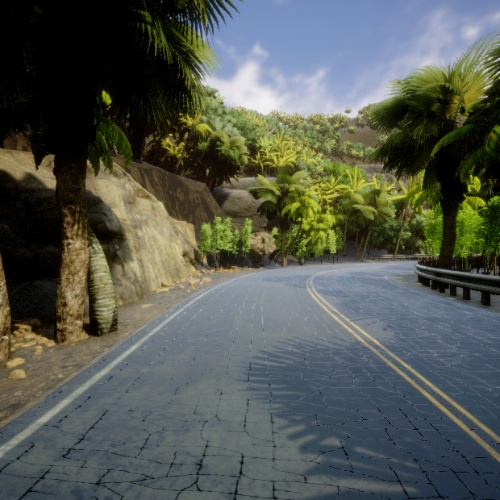
\includegraphics[width=\textwidth]{figs/Diseño/Percepcion/vision_clasica/imagen-original.jpg}
      \caption*{a: Zona curvada}
  \end{minipage}
  \hfill
  \begin{minipage}[t]{0.3\textwidth}
      \centering
      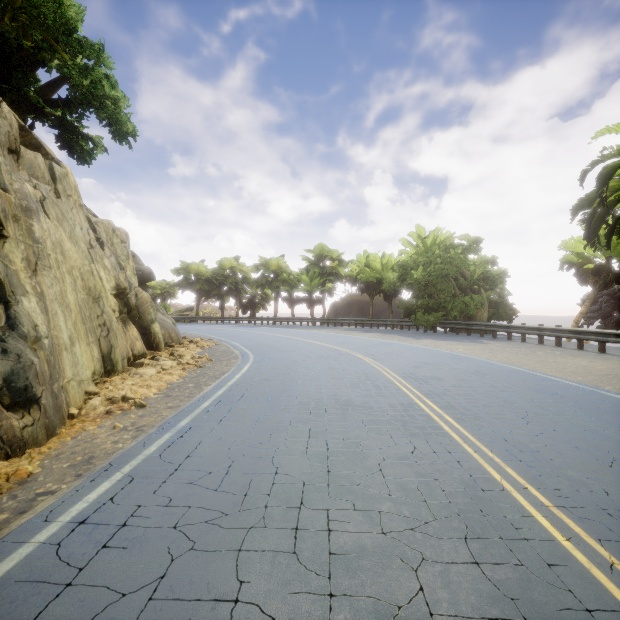
\includegraphics[width=\textwidth]{figs/Diseño/Percepcion/vision_clasica/imagen-original2.jpg}
      \caption*{b: Zona recta}
  \end{minipage}
  \hfill
  \begin{minipage}[t]{0.3\textwidth}
      \centering
      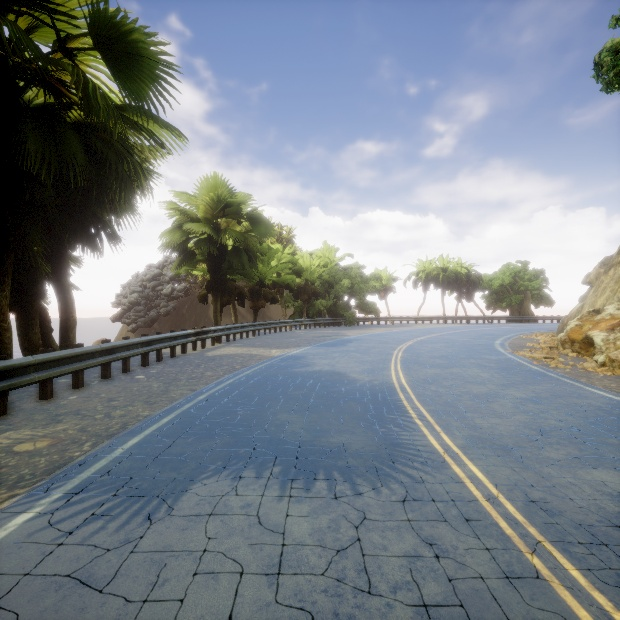
\includegraphics[width=\textwidth]{figs/Diseño/Percepcion/vision_clasica/imagen-original3.jpg}
      \caption*{c: Zona semirecta}
  \end{minipage}
  
  \vspace{1cm}
  
  \begin{minipage}[t]{0.3\textwidth}
      \centering
      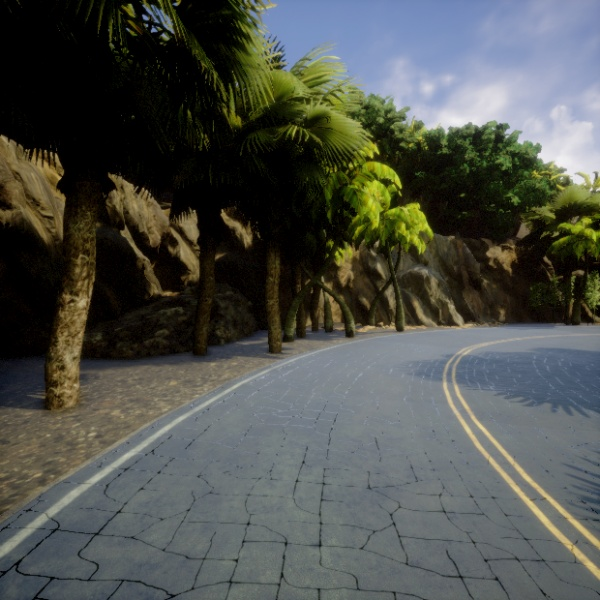
\includegraphics[width=\textwidth]{figs/Diseño/Percepcion/vision_clasica/deteccion.jpg}
      \caption*{d: Detección en la zona curvada}
  \end{minipage}
  \hfill
  \begin{minipage}[t]{0.3\textwidth}
      \centering
      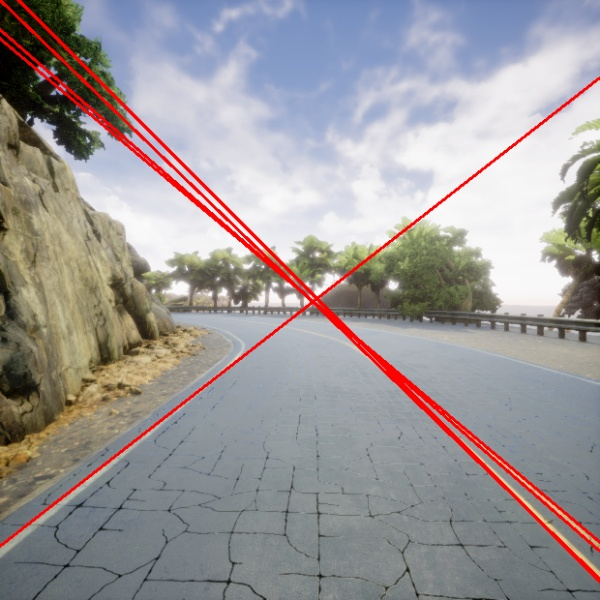
\includegraphics[width=\textwidth]{figs/Diseño/Percepcion/vision_clasica/deteccion2.jpg}
      \caption*{e: Detección en la zona recta}
  \end{minipage}
  \hfill
  \begin{minipage}[t]{0.3\textwidth}
      \centering
      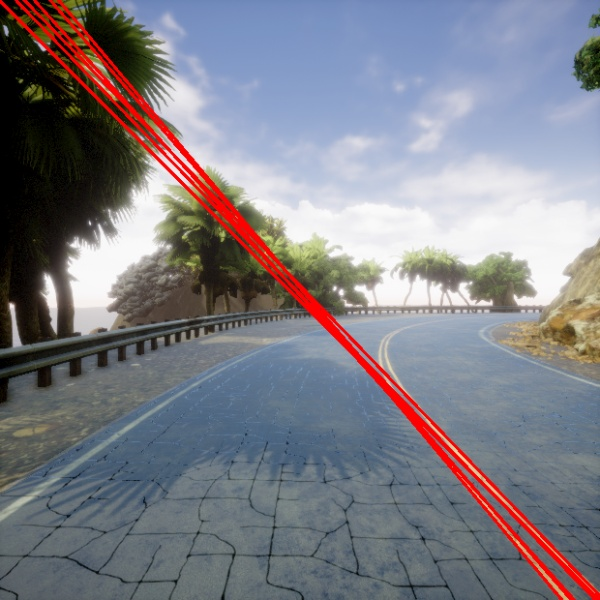
\includegraphics[width=\textwidth]{figs/Diseño/Percepcion/vision_clasica/deteccion3.jpg}
      \caption*{f: Detección en la zona semirecta}
  \end{minipage}
  \caption{Resultado de la detección de líneas utilizando visión clásica}
  \label{Vision_clasica}
\end{figure}

Debido al mal funcionamiento de estos algoritmos de visión clásica en la detección de líneas en los carriles, 
hemos optado por utilizar técnicas de inteligencia artificial, en especial Deep Learning, utilizando la red neuronal YOLOP. Como se comenta en la sección \ref{sec:YOLOP}, 
YOLOP es una red neuronal que realiza una detección de objetos de tráfico, detección del área segmentada transitable y una detección de las líneas que aparecen en las áreas transitables. Es importante 
destacar que se realiza solamente la inferencia de los distintos modelos que ofrece YOLOP, sin realizar un nuevo entrenamiento. Este enfoque nos permite aprovechar 
la detección de las líneas proporcionadas de la red para mejorar la percepción del entorno del dron, proporcionando una detección más robusta y precisa en una variedad de condiciones
de las carreteras urbanas dentro del entorno de Airsim. 

\subsubsection{Inferencia de YOLOP}
\label{sec:Inferencia de YOLOP}

Para realizar la deteción de las líneas en la carretera nos vamos ayudar de la red neuronal YOLOP\footnote{\url{https://github.com/hustvl/YOLOP}}. En primer lugar, 
se realiza la inferencia del modelo End-to-end.pth y más adelante la inferencia de los modelos yolop-320-320.onnx, yolop-640-640.onnx e yolop-1280-1280.onnx mediante el Onnx Runtime. 
El archivo End-to-end.pth es un modelo preentrenado construido en formato Pytorch que contiene los pesos y sesgos de la red neuronal después del entrenamiento. En el contexto de 
redes neruronales, \texttt{end-to-end} significa que la red se entrena para realizar todas las etapas de un proceso completo, para YOLOP, esto significa que se ha entrenado de manera integral 
para realizar simultáneamente todas sus tareas (detección de objetos, segmentación de áreas transitables y detección de líneas). Para poder cargar este modelo, se realiza 
su carga mediante el repositorio de github\footnote{\url{https://github.com/hustvl/YOLOP}}
especificando el modelo de la red neuronal y la opción 'pretrained' colocada con valor True, especificando que los pesos del modelo de la red se cargan del archivo End-to-end.pth.\newline

\begin{code}[h]
  \begin{lstlisting}[language=Python]
  import torch
  model = torch.hub.load('hustvl/yolop', 'yolop', pretrained=True)

  \end{lstlisting}
  \caption[Cargar modelo YOLOP con pesos preentrenados End-to-end.pth]{Cargar modelo YOLOP con pesos preentrenados End-to-end.pth}
  \label{cod:cargar_modelo}
  \end{code}  

Una vez tengamos el modelo cargado del repositorio como se ilustra en el código \ref{cod:cargar_modelo}, se puede escoger 
si se quiere realizar la inferencia mediante el uso de la CPU o el uso de la GPU. Para una mejor optimización de la red neuronal, se utiliza
la GPU para realizar la inferencia asignandole el dispositivo GPU como se muestra en el código \ref{cod:codeloadYOLOP}.\newline

  
\begin{code}[h]
    \begin{lstlisting}[language=Python]
    device = torch.device("cuda" if torch.cuda.is_available() else "cpu")
    model = model.to(device)
  
    \end{lstlisting}
    \caption[Cargar modelo YOLOP escogiendo como disposivo la GPU]{Cargar modelo YOLOP escogiendo como disposivo la GPU}
    \label{cod:codeloadYOLOP}
    \end{code}  

      También esta red neuronal ofrece modelos con formato Onnx: \texttt{Yolop-320-320.onnx, Yolop-640-640.onnx e Yolop-1280-1280.onnx}. Estos modelos son construidos a partir del archivo 
      \texttt{End-to-end.pth} y se convierten en modelos con formato Onnx. Cada modelo proporcionado con formato onnx tiene una resolución distinta de entrada en cuanto a las dimensiones
      de las imágenes. El archivo \texttt{Yolop-320-320.onnx} necesita una entrada con unas dimensiones de 320x320 píxeles en las imágenes, el archivo \texttt{Yolop-640-640.onnx} necesita 
      una entrada con unas dimensiones de 640x640 píxeles en las imágenes y por último el archivo \texttt{Yolop-1280-1280.onnx} se necesita unas dimensiones de imágenes de 1280x1280 píxeles. 
      En cuanto al uso de estos modelos, se debe realizar la configuración de los drivers de CUDA con la versión disponible para Onnx Runtime, 
      dichas versiones tienen que ser compatible entre sí. Para ello nos vamos a guiar mediante la tabla requisitos de la página oficial de Onnx Runtime\footnote{\url{https://onnxruntime.ai/docs/execution-providers/CUDA-ExecutionProvider.html}}. \newline
      Cuando se trabaja con Onnx Runtime, se puede especificar qué proveedores de ejecución utilizar para ejecutar la inferencia del modelo de Onnx que se escoja. Cada proveedor 
      contiene un conjunto de núcleos optimizados para un objetivo específico (por ejemplo, CPU, GPU, IoT), cada proveedor se especifica en una lista en orden de prioridad. Para realizar 
      inferencia de estos modelos, se escoge CUDA para ejecutar mediante la GPU. En el código \ref{yolop320} se muestra la carga del modelo Yolop-320-320.onnx junto con la configuración
      del provider CUDAExecutionProvider. 
      
      \begin{code}[h]
        \begin{lstlisting}[language=Python]
          import onnxruntime as ort

          ROUTE_MODEL = "/home/bb6/YOLOP/weights/yolop-320-320.onnx"
          ort_session = ort.InferenceSession(ROUTE_MODEL,providers=['CUDAExecutionProvider'])
      
        \end{lstlisting}
        \caption[Cargar modelo]{Cargar modelo por ejemplo YOLOP-320-320.onnx}
        \label{yolop320}
        \end{code}  

        Para realizar la redimensión de las imágenes dependiendo de cada modelo, se utiliza un método implementado por ellos 
        que se puede encontrar en la siguiente página\footnote{\url{https://debuggercafe.com/yolop-onnx-inference-on-cpu}}, el cuál redimensiona la imagen de entrada según cada modelo. En el código 
        \label{cod:Inferencia_onnx} se realiza la inferencia del modelo Yolop-320-320.onnx. 

        \begin{code}[h]
          \begin{lstlisting}[language=Python]
            _, da_seg_out, ll_seg_out = self.ort_session.run(
              ['det_out', 'drive_area_seg', 'lane_line_seg'],
              input_feed={"images": img}
          )
        
          \end{lstlisting}
          \caption[Inferencia del modelo yolop-320-320.onnx]{Inferencia del modelo yolop-320-320.onnx}
          \label{cod:Inferencia_onnx}
          \end{code}  

        La inferencia del resto de modelos de Onnx se realizan de la misma forma pero teniendo en cuenta que se tendrá que cambiar las dimensiones de las imágenes de entrada y la ruta
        en donde se almacena dicho modelo. \newline

        Por último, para poder utilizar imágenes en la inferencia de YOLOP tanto del modelo de Pytorch como de los modelos de Onnx, se debe convertir la imagen en un tensor. Para poder realizarlo, se utiliza la función transforms.toTensor\footnote{\url{https://pytorch.org/vision/main/generated/torchvision.transforms.ToTensor.html}} 
        para realizar la transformación a tensor. Una vez se obtenga el tensor, se puede realizar la inferencia del modelo end-to-end.pth como se ilustra en el código \ref{cod:Inferencia}.
    
        \begin{code}[h]
          \begin{lstlisting}[language=Python]
         
            from torchvision import transforms
    
            transform = transforms.ToTensor() 
                        
          imagen_tensor = transform(cv_image).to(device).unsqueeze(0)
          _, da_seg_out, ll_seg_out = self.model(imagen_tensor)
        
          \end{lstlisting}
          \caption[Inferencia del modelo]{Inferencia del modelo en Pytorch}
          \label{cod:Inferencia}
          \end{code}  
    
        Como resultado de la inferencia se obtiene un tensor de salida que corresponde a la probabilidad de detección de la segmentación
        y la detección de las líneas de la calzada. Dicho tensor se debe de convertir en una imagen para poder visualizar
        dicho resultado como una imagen. 
        Por ello, se convierte el tensor en un array numpy y se realiza una transformacion para cambiar las dimensiones de (H,W,C) 
        a (C,H,W) esto se realiza ya que en OpenCV se representan imágenes en formato numpy array y se transpone las dimensiones\footnote{\url{https://lindevs.com/convert-pytorch-tensor-to-opencv-image-using-python}}. 
    
        Después de este proceso, se obtiene un array de numpy que se normaliza con valores de 0-1. Con la normalización 
        se ayuda a igualar la escala de los píxeles de la imagen. Finalmente se muestra el resultado de la inferencia de la red 
        en una imagen como se ilustra en el código \ref{cod:Resultadoinferencia}. Al normalizar los valores de 0-1, los píxeles con un valor 1 se muestran en la imagen final, asignándoles 
        color verde el resultado de la segmentación de la calzada y de color rojo la detección de las líneas de la calzada. \newline
    
        \begin{code}[H]
          \begin{lstlisting}[language=Python]
            import cv2
            import numpy as np
            for image in (da_seg_out,ll_seg_out):
              image_np = image.detach().cpu().numpy()
              image_array = np.transpose(image_np, (2, 3, 1, 0))
    
              image_norm = cv2.normalize(image_array[:,:,1,:], None, 0,1, cv2.NORM_MINMAX, cv2.CV_8U)
    
              images.append(image_norm)
    
            cv_image[images[0] == 1] = [0, 255, 0]
            cv_image[images[1] == 1] = [0, 0, 255]
    
            cv2.imshow('Image', cv_image)
            cv2.waitKey(1)
          \end{lstlisting}
          \caption[Resultado de la inferencia del modelo YOLOP]{Inferencia de YOLOP mediante los pesos End-to-end.pth}
          \label{cod:Resultadoinferencia}
          \end{code}  


\subsubsection{Resultados de YOLOP }
\label{sec:resultados}
En esta sección se constrastan los resultados de la inferencia de YOLOP con los diferentes modelos que ofrece esta red. Para realizar esta comparación, se uso el ordenador 
PC2 junto con la GPU Nvidia 2070 RTX para realizar la inferencia de cada modelo. Se recopilan datos del tiempo medio de inferencia en milisegundos de cada 
modelo de YOLOP durante aproximadamente
un mínuto, mientras se teleopera el dron por las carreteras. El objetivo de este análisis es determinar qué modelo ofrece mejores resultados en términos de eficiencia y rendimiento. 
En la figura \ref{fig:resultados_pesos_preentrenados} se muestra este análisis mostrando la media en realizar la inferencia de YOLOP utilizando los modelos 
End-to-end.pth, Yolop-320-320.onnx, Yolop-640-640.onnx e Yolop-1280-1280.onnx en milisegundos.

El modelo que tiene una inferencia menor al resto se trata de Yolop-320-320.onnx, tiene un tiempo de inferencia alrededor de 10 milisegundos, esto
significa que el modelo Yolop-320-320.onnx tiene aproximadamente un rate de 100 FPS. Si comparamos este resultado con los restantes modelos, es el ganador en cuanto 
en tiempo de inferencia, rate y mejores resultados. 
Onnx está diseñado para ser más eficiente en términos de memoria y velocidad de inferencia en cuanto Pytorch, lo que puede mejorar la velocidad y la precisión
del modelo, una menor resolución en cuanto al tamaño de las imágenes reduciendo la cantidad de información al procesarlas. Aun así, depende de varios factores y según las necesidades, 
en este caso se busca un equilibrio entre velocidad de inferencia y mejores resultados en cuanto a la detección de las líneas de la calzada. 

\begin{figure} [H]
  \begin{center}
    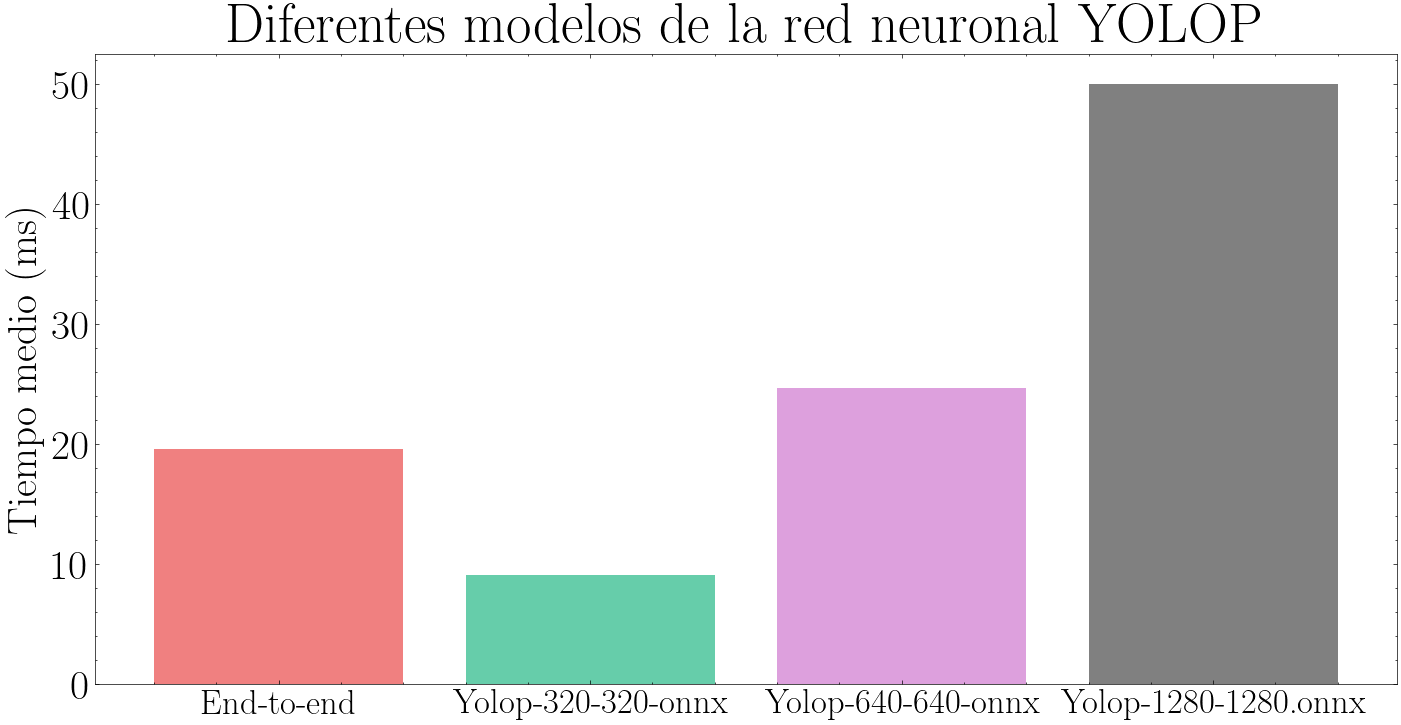
\includegraphics[scale=0.4]{figs/Diseño/YOLOP/comparativa.png}
  \end{center}
  \caption{Resultados de los diferentes modelos que ofrece la red YOLOP}
  \label{fig:resultados_pesos_preentrenados}
\end{figure}\

Por ello, se escoge el modelo Yolop320-320.onnx ya que obtiene mejores resultados para poder realizar la detección de las líneas del carril. 
En cuanto a los resultados de la inferencia, en la figura \ref{f:resultadosYOLOP} 
se puede observar los diferentes resultados que tiene la red neuronal YOLOP dependiendo de qué modelo utilizar. Para ello, se utiliza dos zonas totalmente distintas para realizar 
la inferencia de los modelos. Aunque se escoja el modelo Yolop-320-320.onnx, la detección de las líneas no es perfecta como se muestra en la figura 
\ref{f:Inferencia320-320}.
\begin{figure} [H]
  \begin{center}
    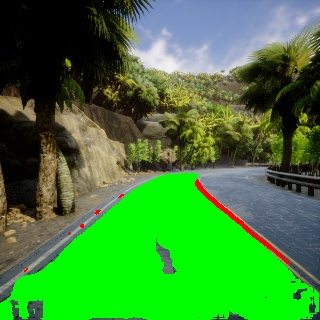
\includegraphics[scale=0.6]{figs/Diseño/YOLOP/resultados-yolop/sitio3/yolop-320-320.jpg}
  \end{center}
  \caption{Resultados de la inferencia del modelo yolop-320-320.onnx}
  \label{f:Inferencia320-320}
\end{figure}\

Depende de como se halla 
entrenado la red neuronal. Para poder llegar a escoger qué líneas necesitamos del carril que queremos seguir, utilizaremos un algoritmo de aprendizaje automático llamado clustering, 
en especial, DBSCAN. En donde, se realiza un post-procesado de las líneas detectadas por parte del modelo Yolop-320-320.onnx para utilizarlas en el algoritmo de DBSCAN y poder 
construir el carril a partir de regresiones cuadráticas.



\begin{figure} [H]
  \begin{center}
    \includegraphics[scale=0.06]{figs/Diseño/YOLOP/resultados.png}
  \end{center}
  \caption{Resultados de los diferentes modelos de la red neuronal YOLOP}
  \label{Resultados de los diferentes modelos de la red neuronal YOLOP}
\end{figure}\

\subsubsection{DBSCAN}
\label{sec:DBSCAN}

Para saber qué líneas detectadas por parte del modelo Yolop320-320.onnx se seleccionarán, se utiliza un algoritmo de aprendizaje no supervisado llamado clustering, en particular
DBSCAN(Density-Based Spatial Clustering of Applications with Noise)\cite{ski_dbs}.\newline

Dicho algoritmo contiene varios parámetros que son importantes conocerlos y configurarlos: 
\begin{enumerate}
  \item \textbf{Eps}: Consiste en la distancia máxima que puede existir entre dos muestras para que una se considere vecina de la otra. Dicha distancia no se trata de un límite 
  máximo entre las distancias que puede haber dentro de un cluster.
  \item \textbf{Min\_samples}: Es el número mínimo de muestras dentro de un vecindario para que un punto se considere como un punto central incluyendo al propio punto.
  \item \textbf{Metric}: La métrica utilizada para calcular la distancia entre los conjuntos de clústeres (por defecto es la distancia euclidiana). 
\end{enumerate}
Los valores de los parámetros de la distancia máxima y el número mínimo de muestras se deben elegir cuidadosamente, es decir, si colocamos una distancia 
máxima alta puede provocar que los clústeres que queramos que pertenezcan a un distinto grupo pertenezcan al mismo grupo. 
Si min\_samples se establece en un valor alto, DBSCAN encontrará clústeres más densos y 
si se establece en un valor bajo, los clústeres encontrados serán más dispersos. \newline
Para entender como funciona el algoritmo, en la figura \ref{fig:Ejemplo_DBSCAN} recogida por este artículo\cite{DBSCAN} se ilustra 
un ejemplo teniendo un número de muestras ubicadas aproximadamente cercanas unas de otras. Aplicamos el algoritmo de DBSCAN 
teniendo como valor el número mínimo de muestras 3, eso significa que para que se considere una muestra a un grupo de cluster tendrá que tener una densidad de 3. El algoritmo itera por
las muestras y compara el valor de la distancia máxima y el número mínimo de muestras. 
Si ningún de estos dos parámetros no se cumpliese ya que puede darse que una muestra se encuentra lejana del grupo de muestras será etiquetado como ruido, esto quiere decir
que no pertenecerá a ningún grupo de clústeres. El resultado del algoritmo ha catalogado dos grupos de clústeres y 3 muestras. \newline

\begin{figure} [H]
  \begin{center}
    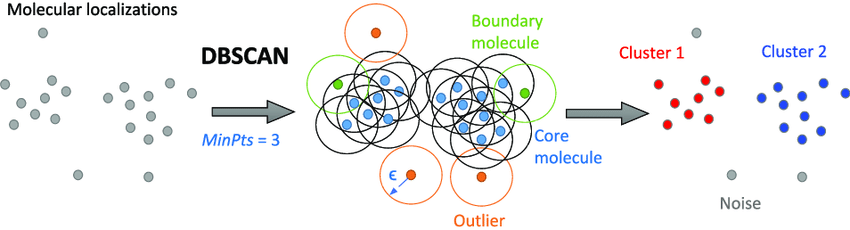
\includegraphics[scale=0.5]{figs/Diseño/DBSCAN/DBSCAN-Illustration.png}
  \end{center}
  \caption{Ejemplo ilustrativo de como funciona el algoritmo de DBSCAN \cite{DBSCAN}}
  \label{fig:Ejemplo_DBSCAN}
\end{figure}\

Por lo que para encontrar los valores de estos dos parámetros durante el desarrollo del TFG fue experimental y quedándonos con el mejor resultado. La distancia máxima tiene un valor de 10 
y el número mínimo de muestras son de 5 muestras. Lo que significa que la distancia máxima que tienen los puntos para pertenecer al mismo grupo de clústeres es de 10 de distancia en pixeles
con un mínimo de muestras pertenecientes de 5 muestras como se muestra en el código \ref{cod:DBSCAN}. Para poder aplicar este algoritmo a partir del resultado de la imagen de la red neuronal se convierte la imagen resultante
de la red neuronal en un array bidimensional de coordenadas x e y de puntos con la ayuda de la función de numpy column\_stack\footnote{\url{https://numpy.org/doc/stable/reference/generated/numpy.column_stack.html}}, 
transformando un array simple de una dimensión a un array de dos dimensiones. Una vez se realice lo anterior, se obtiene un array bidimensional listo para el algoritmo DBSCAN .\newline

El resultado de DBSCAN es una lista con etiquetas de 0 a n, siendo 0 el primer grupo de clusters detectado y 
n el último grupo de clusters detectado. De las listas de etiquetas se eliminan los clusters que hallan sido etiquetados como ruido (-1). Para obtener el resultado solamente basta con iterar en dicha lista y mostrar los puntos correspondientes de cada etiqueta en la imagen de salida.
Visualmente se puede apreciar en la figura \ref{f:Rresultadosdbscan} los diferentes resultados que tiene este algoritmo en localizaciones distintas. 


\begin{figure}[H]
  \centering
  \begin{minipage}[t]{0.3\textwidth}
      \centering
      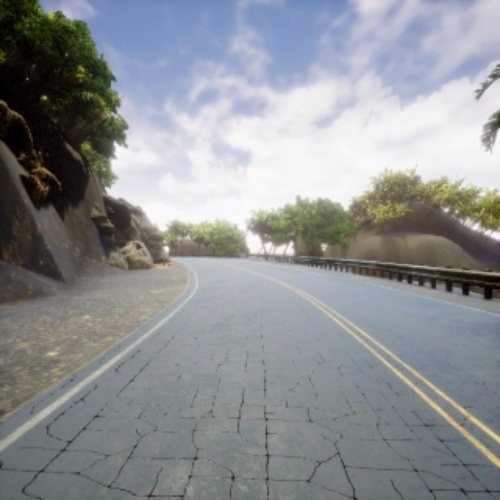
\includegraphics[width=\textwidth]{figs/Diseño/DBSCAN/comparativa/dbscan1-original.jpg}
      \caption*{a: Zona curvada}
  \end{minipage}
  \hfill
  \begin{minipage}[t]{0.3\textwidth}
      \centering
      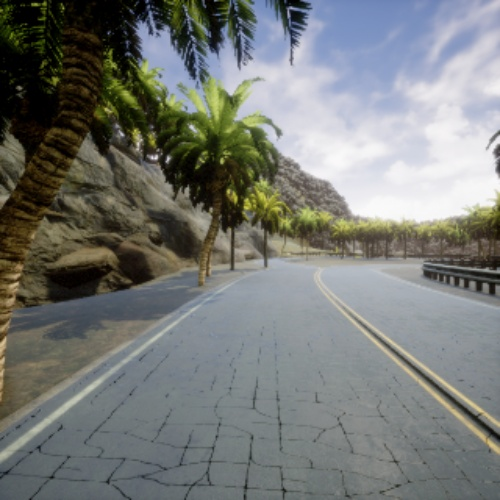
\includegraphics[width=\textwidth]{figs/Diseño/DBSCAN/comparativa/dbscan2-original.jpg}
      \caption*{b: Zona recta}
  \end{minipage}
  \hfill
  \begin{minipage}[t]{0.3\textwidth}
      \centering
      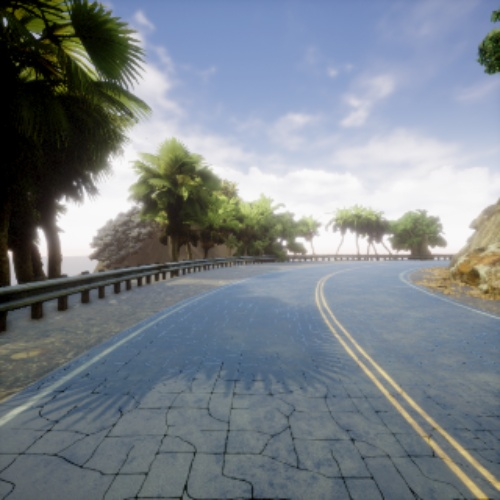
\includegraphics[width=\textwidth]{figs/Diseño/DBSCAN/comparativa/dbscan4-original.jpg}
      \caption*{c: Zona semirecta}
  \end{minipage}
  
  \vspace{1cm}
  
  \begin{minipage}[t]{0.3\textwidth}
      \centering
      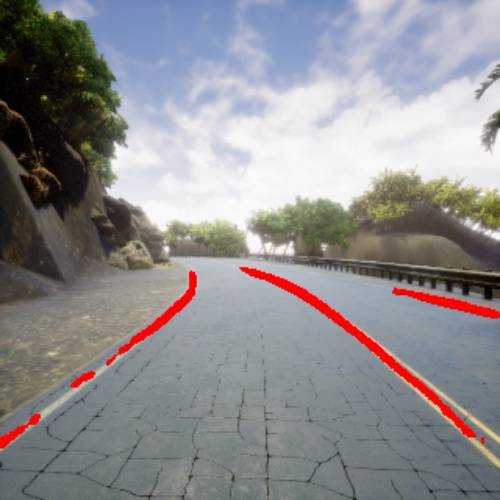
\includegraphics[width=\textwidth]{figs/Diseño/DBSCAN/comparativa/yolop1.jpg}
      \caption*{d: Detección en la zona curvada}
  \end{minipage}
  \hfill
  \begin{minipage}[t]{0.3\textwidth}
      \centering
      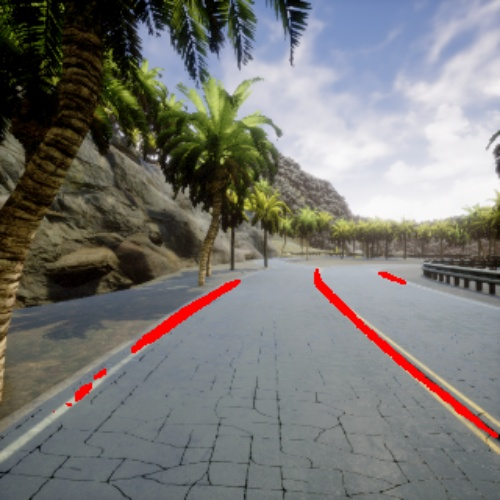
\includegraphics[width=\textwidth]{figs/Diseño/DBSCAN/comparativa/yolop2.jpg}
      \caption*{e: Detección en la zona recta}
  \end{minipage}
  \hfill
  \begin{minipage}[t]{0.3\textwidth}
      \centering
      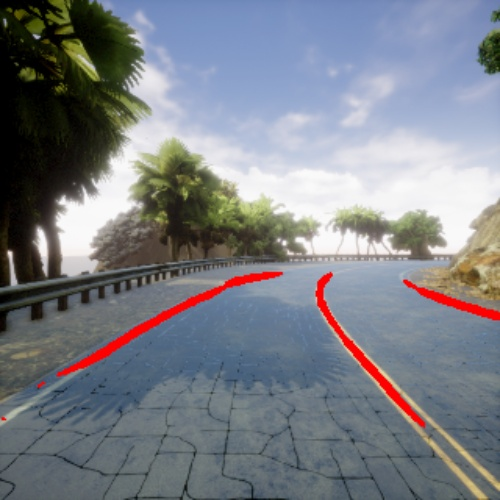
\includegraphics[width=\textwidth]{figs/Diseño/DBSCAN/comparativa/yolop3.jpg}
      \caption*{f: Detección en la zona semirecta}
  \end{minipage}

  \vspace{1cm}
  
  \begin{minipage}[t]{0.3\textwidth}
      \centering
      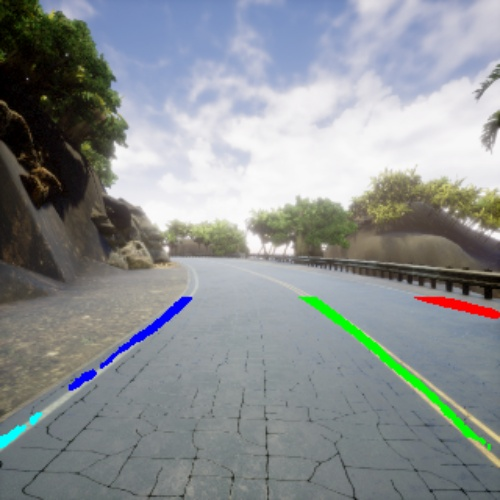
\includegraphics[width=\textwidth]{figs/Diseño/DBSCAN/comparativa/dbscan1.jpg}
      \caption*{d: Detección en la zona curvada}
  \end{minipage}
  \hfill
  \begin{minipage}[t]{0.3\textwidth}
      \centering
      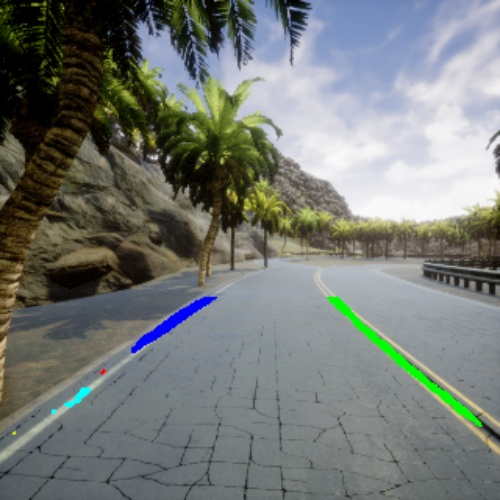
\includegraphics[width=\textwidth]{figs/Diseño/DBSCAN/comparativa/dbscan2.jpg}
      \caption*{e: Detección en la zona recta}
  \end{minipage}
  \hfill
  \begin{minipage}[t]{0.3\textwidth}
      \centering
      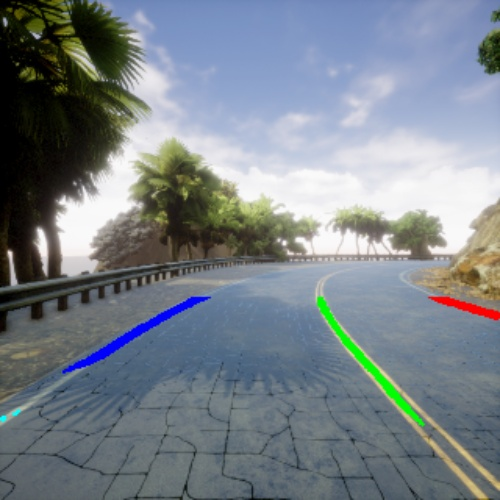
\includegraphics[width=\textwidth]{figs/Diseño/DBSCAN/comparativa/dbscan4.jpg}
      \caption*{f: Detección en la zona semirecta}
  \end{minipage}
  \caption{Resultado de la detección de líneas utilizando visión clásica}
  \label{Vision_clasica}
\end{figure}



\begin{code}[h]
  \begin{lstlisting}[language=Python]
    def clustering(self,cv_image):
    
    points_lane = np.column_stack(np.where(cv_image > 0))
    dbscan = DBSCAN(eps=10, min_samples=5,metric="euclidean")

    if points_lane.size > 0:
        dbscan.fit(points_lane)
        labels = dbscan.labels_

        clusters = set(labels)
        if -1 in clusters:
            clusters.remove(-1)
    
        for cluster in clusters:
            points_cluster = points_lane[labels==cluster,:]
            centroid = points_cluster.mean(axis=0).astype(int)
            color = self.colors[cluster % len(self.colors)]
            cv_image[points_cluster[:,0], points_cluster[:,1]] = color

        return cv_image
  
  \end{lstlisting}
  \caption[Algoritmo de custering utilizando DBSCAN]{Algoritmo de clustering utilizando DBSCAN}
  \label{cod:DBSCAN}
  \end{code}  


\subsubsection{Filtrado de clústeres}
\label{clasificación:cluster}
Una vez realizado el algoritmo de DBSCAN necesitamos quedarnos con el grupo de clústeres que pertenezcan al carril que queremos seguir. Para conseguirlo, se calcula los centroides de cada
grupo de clústeres detectado y los clasificaremos en función de sí se encuentran en la derecha o izquierda respecto al centro de la imagen. La imagen tiene unas dimensiones de 320x320 píxeles, 
siendo su centro (160,160) pixeles, x = 160 e y = 160. Nos fijaremos solamente en los valores de x de los centroides para poder clasificarlos en función del centro de la 
imagen, a partir de ello serán divididos en dos grupos distinguidos: derecha e izquierda de la imagen como se muestra en el código \ref{cod:Clasificación de clústeres}. \newline

\begin{code}[h]
  \begin{lstlisting}[language=Python]
    # Check if the centroid is within the desired lane

    WIDTH = cv_image.shape[1]
    if centroid[1] < WIDTH/2:  # left lane
        left_clusters.append((points_cluster,centroid))
       
    elif centroid[1] >= WIDTH/2:  # right lane
        right_clusters.append((points_cluster, centroid))
       
  
  \end{lstlisting}
  \caption[Clasificación de clústeres según las dimensiones de la imagen ]{Clasificación de clústeres respecto a las dimensiones de la imagen}
  \label{cod:Clasificación de clústeres}
  \end{code}  


Cuando sean clasificados los grupos de los clústeres, necesitamos quedarnos con qué subgrupo de cada grupo de clústeres (izquierda e derecha) nos queremos quedar respecto al carril. Esogemos dichos grupos mediante una función máximizada 
respecto a un punto central P predefinido con valor (220,160) siendo 220 el valor de las y e 160 el valor de las x, dichos valores son calculados respecto 
a las dimensiones de la imagen 320x320 píxeles. Es importante mencionar que cuando trabajamos con puntos en numpy las coordenadas estan opuestas, es decir, en vez de tener el formato (x,y) como estamos acostumbrados a trabajar tienen el formato(y,x). 
A parte de escoger lo sugrupos respecto a un punto central P también se realiza en función de la densidad de puntos de dicho grupo de clústeres de la derecha u izquierda detectados, 
con esto conseguimos que no solamente se escoja en función de la cercania si no que también lo haremos según la cantidad de puntos. El proceso se ilustra 
en el código \ref{cod:funcion_maximizada}.\newline

\begin{code}[h]
  \begin{lstlisting}[language=Python]
    def score_cluster(self,cluster, center):
      points_cluster, centroid = cluster
    
      proximity = np.linalg.norm(centroid - center)
      density = len(points_cluster)
      return density / proximity

  \end{lstlisting}
  \caption[Función maximizada para escoger el grupo de cluster más cercano y denso respecto al punto P]{Función maximizada para escoger el grupo de cluster más cercano y denso respecto al punto P}
  \label{cod:funcion_maximizada}
  \end{code}  

  En la figura \ref{fig:DBSCAN_imagen} se muestra todo el proceso desde el uso del algoritmo de DBSCAN hasta la clasificación de clústeres respecto al carril 
  representados en color verde y rojo. Después de tener la clasificación de los grupos de clústeres se procede a realizar dos regresiones cuadráticas para construir las líneas del carril que queremos seguir.


  \begin{figure}[H]
    \centering
    \begin{minipage}{0.3\textwidth}
      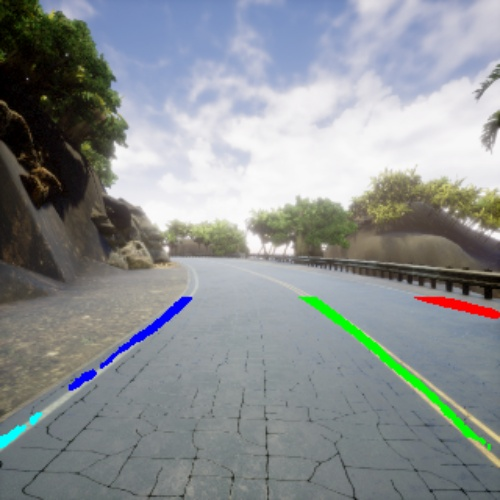
\includegraphics[width=\linewidth]{figs/Diseño/DBSCAN/comparativa/dbscan1.jpg}
    \end{minipage}
    \hfill
    \begin{minipage}{0.3\textwidth}
      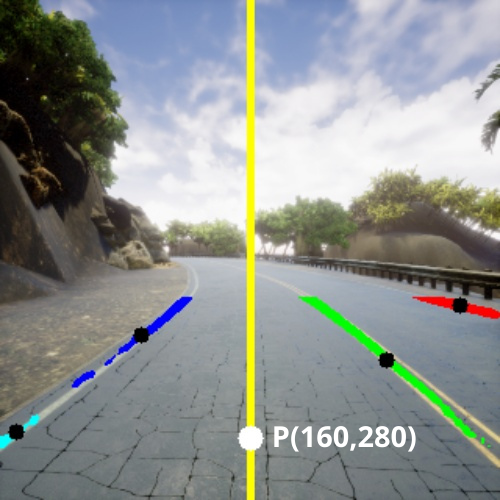
\includegraphics[width=\linewidth]{figs/Diseño/DBSCAN/clustering_centroids.png}
    \end{minipage}
    \hfill
    \begin{minipage}{0.3\textwidth}
      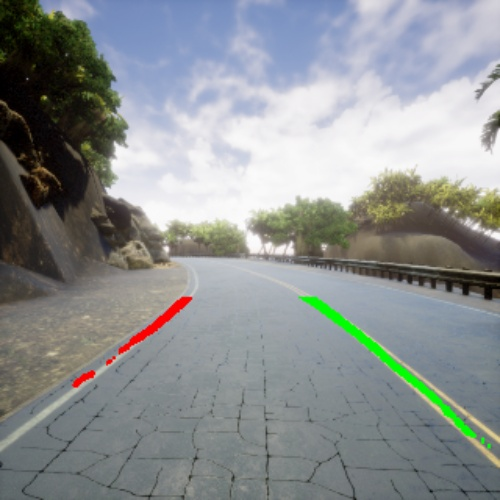
\includegraphics[width=\linewidth]{figs/Diseño/DBSCAN/filter_clustering.jpg}
    \end{minipage}
    \caption{Proceso de selección de las líneas del carril}
    \label{fig:comparativa}
  \end{figure}

\subsection{Regresión cuadrática}
\label{sec:Regresión cuadrática}
Como anteriormente hemos mencionado, cuando se clasifique los clústeres correctamente daremos pie a la construcción de dos regresiones cuadráticas. \newline 

La regresión es un método de aprendizaje supervisado el cual consiste en aproximar un número N de puntos a una recta, curva, etc, en nuestro caso hemos escogido realizar una regresión cuadrática ya que el recorrido
que vamos a realizar las líneas detectadas por la red neuronal no son totalmente rectas si no que se tratan de líneas curvilíneas por lo que la regresión cuadrática en este papel puede 
funcionar perfectamente. 
Para la construcción de las regresiones cuadráticas se utiliza las funciones de la librería numpy denominada Polyfit\footnote{\url{https://numpy.org/doc/stable/reference/generated/numpy.polyfit.html}}
y Polyval\footnote{\url{ https://numpy.org/doc/stable/reference/generated/numpy.polyval.html}}. 
Polyfit es una función que calcula los coeficientes del polinomio que mejor se ajusta a los datos utilizando el método de los mínimos 
cuadrados para la ecuación cuadrática,obteniendo tres coeficientes, denominados a,b y c. Definimos los valores de las coordenadas x como los puntos que queremos
realizar dicho calculo, se realiza un rango entre un mínimo y un máximo ajustándolo a las dimensiones de la imagen, además de 
ayudarnos con dos puntos auxiliares en los extremos inferiores en el cálculo de la regresión como se muestra en el código \ref{cod:Calculocoeficientes}.
 \newline

\begin{code}[H]
  \begin{lstlisting}[language=Python]
  
    FACTOR_PIXEL = 20
    MIN_VALUE_X = (cv_image.shape[1] // 2) + FACTOR_PIXEL
    MAX_VALUE_X = cv_image.shape[1]
  
    valuesX = np.arange(MIN_VALUE_X,MAX_VALUE_X) 
    point = np.array([cv_image.shape[1]/1.104,cv_image.shape[1]])
    coefficients = np.polyfit(points_cluster[:,0],points_cluster[:,1],2)
  \end{lstlisting}
  \caption[Calculo de los coeficientes]{Cálculo de los coeficientes de la regresión cuadrática}
  \label{cod:Calculocoeficientes}
  \end{code}  

Con dichos coeficientes se realiza una media de los últimos diez valores como se ilustra en el código \ref{cod:regresión} y por cada cinco iteraciones dicha media se volverá a calcular, este paso lo realizamos ya que 
queremos disminuir las oscilaciones causadas de las detecciones de la red neuronal que son cruciales a la hora de realizar el comportamiento sigue carril. Una vez calculados los coeficientes, se calcula la regresión cuadrática mediante la función Polyval, dicha función calcula
la función cuadrática con los coeficientes calculados anteriormente. \newline 
Cuando se obtiene los valores de la función cuadrática, se realiza una clasificación para quedarnos con los puntos obtenidos
de dicha función los que se encuentren en el eje y entre los valores 0 hasta el máximo de la imagen mneos una unidad que sería 319, esto se debe hacer ya que dicha función como resultado puede 
dar números negativos realizando dicha regresión además de que en una imagen no se puede indexar con números negativos. \newline

\begin{code}[H]
  \begin{lstlisting}[language=Python]

    self.list_coeff_a.append(coefficients[0])
    self.list_coeff_b.append(coefficients[1])
    self.list_coeff_c.append(coefficients[2])

    a = np.mean(self.list_coeff_a[-10:])
    b = np.mean(self.list_coeff_b[-10:])
    c = np.mean(self.list_coeff_c[-10:])

    mean_coeff = np.array([a,b,c])

    self.counter += 1

    if(self.counter > 5):
      self.list_coeff_a.clear()
      self.list_coeff_b.clear()
      self.list_coeff_c.clear()  


    values_fy = np.polyval(mean_coeff,valuesX).astype(int)
    fitLine_filtered = [(x, y) for x, y in zip(valuesX, values_fy) if 0 <= y <= (cvimage.shape[1] - 1)]
    line = np.array(fitLine_filtered)
   

  \end{lstlisting}
  \caption[Cálculo de la regresión cuadrática]{Cálculo de la regresión cuadrática}
  \label{cod:regresión}
  \end{code}  

Este proceso se realiza dos veces, una regresión cuadrática para el grupo de clústeres detectados escogidos de la derecha y otra regresión cuadrática para el grupo de clústeres detectados
escogidos de la izquierda. \newline
Finalmente, con dichas regresiones cuadráticas se procede a realizar una dilatación de los puntos para tener un resultado más llamativo y visual al poder
ver las regresiones cuadráticas como se muestra en la figura \ref{fig:regresión cuadrática}.\newline

\begin{figure} [H]
  \begin{center}
    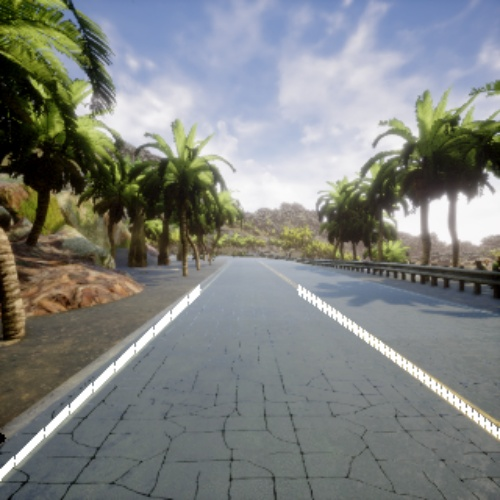
\includegraphics[scale=0.5]{figs/Diseño/Regresiones/Regresiones.jpg}
  \end{center}
  \caption{Resultado de la regresión cuadrática}
  \label{fig:regresión cuadrática}
\end{figure}\

\subsection{Interpolación y cálculo del centro de masas del carril}
\label{sec:Interpolación y cálculo del centro de masas del carril}

Para poder saber qué puntos se encuentran dentro de ambas regresiones cuadráticas, se realiza una interpolación. La interpolación consiste en recorrer
los puntos de la imagen original y quedarnos con los puntos que se encuentren dentro de los límites de ambas regresiones. Se realiza dos interpolaciones, una interpolación para 
los puntos de la regresión de la  derecha
y otra interpolación para los puntos de la regresión izquierda. Estas funciones interpolan los valores de los puntos en y en función de los valores de los puntos en x, más adelante se evalúa los valores de las puntos que se encuentran entre 
ambas regresiones cuadráticas como se muestra en el código \ref{cod:interpolación}. Cuando se proceda a dicha evaluación, se desarrolla un filtro para seleccionar el rango de puntos que representar un fragmento del carril de color azul en la imagen
final. Visualizando el resultado en la figura \ref{fig:interpolación} \newline

\begin{code}[h]
  \begin{lstlisting}[language=Python]

    def interpolate_lines(self,cvimage,points_line_left,points_line_right):


    gray_image = cv2.cvtColor(cvimage, cv2.COLOR_BGR2GRAY) 

    np_gray = np.array(gray_image)

    x, y = np.nonzero(np_gray)


    img_points = np.column_stack((x, y))

    f1 = interp1d(points_line_left[:, 0], points_line_left[:, 1],kind='slinear',fill_value="extrapolate")
    f2 = interp1d(points_line_right[:, 0], points_line_right[:, 1],kind='slinear',fill_value="extrapolate") 
    y_values_f1 = f1(img_points[:, 0])
    y_values_f2 = f2(img_points[:, 0])
    indices = np.where((y_values_f1 < img_points[:, 1]) & (img_points[:, 1] <= y_values_f2))
    
    
    points_between_lines = img_points[indices]
    filtered_points_between_lines = points_between_lines[points_between_lines[:,0] > 180]
    return filtered_points_between_lines
    

  \end{lstlisting}
  \caption[Método de interpolación]{Método del cálculo de las funciones de interpolación}
  \label{cod:interpolación}
  \end{code}  



  \begin{figure} [H]
    \begin{center}
      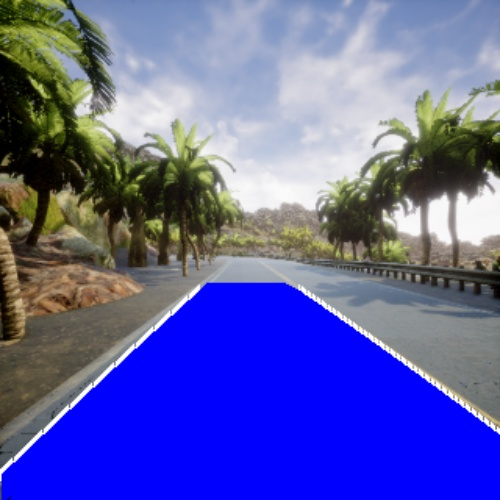
\includegraphics[scale= 0.5]{figs/Diseño/Regresiones/Interpolacion.jpg}
    \end{center}
    \caption{Resultado de la interpolación}
    \label{fig:interpolación}
  \end{figure}\

  Finalmente, cuando obtengamos el cálculo del carril que queremos seguir solamente faltará calcular el centro de masas de dicho fragmento conocido como el centroide siguiendo la ecuación
  del cálculo de centro de masas de una superficie: \newline
  

  \begin{equation} 
    \vec{r}_{CM} = \frac{\sum_{i}m_{i} \vec{r}_{i}}{\sum_{i}m_{i}} = \frac{\sum_{i}m_{i} \vec{r}_{i}}{M} 
    \newline
  \end{equation} 
  \newline
  Supondremos que todos los puntos tienen la misma masa (m\_i = 1). Esto simplifica el cálculo, pero en aplicaciones del mundo real, las masas pueden variar.
  El segundo paso es el cálculo de la masa total, se calcula multiplicando la masa individual (m\_i) por la cantidad de puntos en el carril. A continuación se calcula
  la suma de las posiciones de los puntos ponderadas por su masa y dividimos por la masa total calculada anteriormente. El resultado es una centro de masas conocido como centroide
  con coordenada x e y como se muestra en la figura final \ref{fig:centro de masas}. \newline

  \begin{figure} [H]
    \begin{center}
      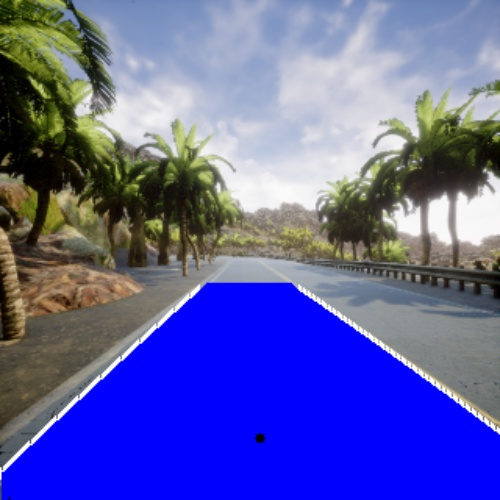
\includegraphics[scale=0.5]{figs/Diseño/Regresiones/centroide.jpg}
    \end{center}
    \caption{Resultado del centro de masas}
    \label{fig:centro de masas}
  \end{figure}\

  \subsection{Análisis del algoritmo de percepción}
  \label{sec:Análisis del algoritmo de percepción}
  Por último, realizamos un analisis de tiempos de cada parte para saber cuánto tiempo tarda en realizarse la percepción completa. Dicho análisis se llama profiling, con esta técnica 
  nos ayuda ver el rendimiento que podemos llegar a tener del algoritmo de percepción en cuanto a eficiencia. En la figura \ref{fig:centro de masas}, 
  se muestra una media de cuanto tarda cada componente de la percepción en segundos.


  \begin{figure} [H]
    \begin{center}
      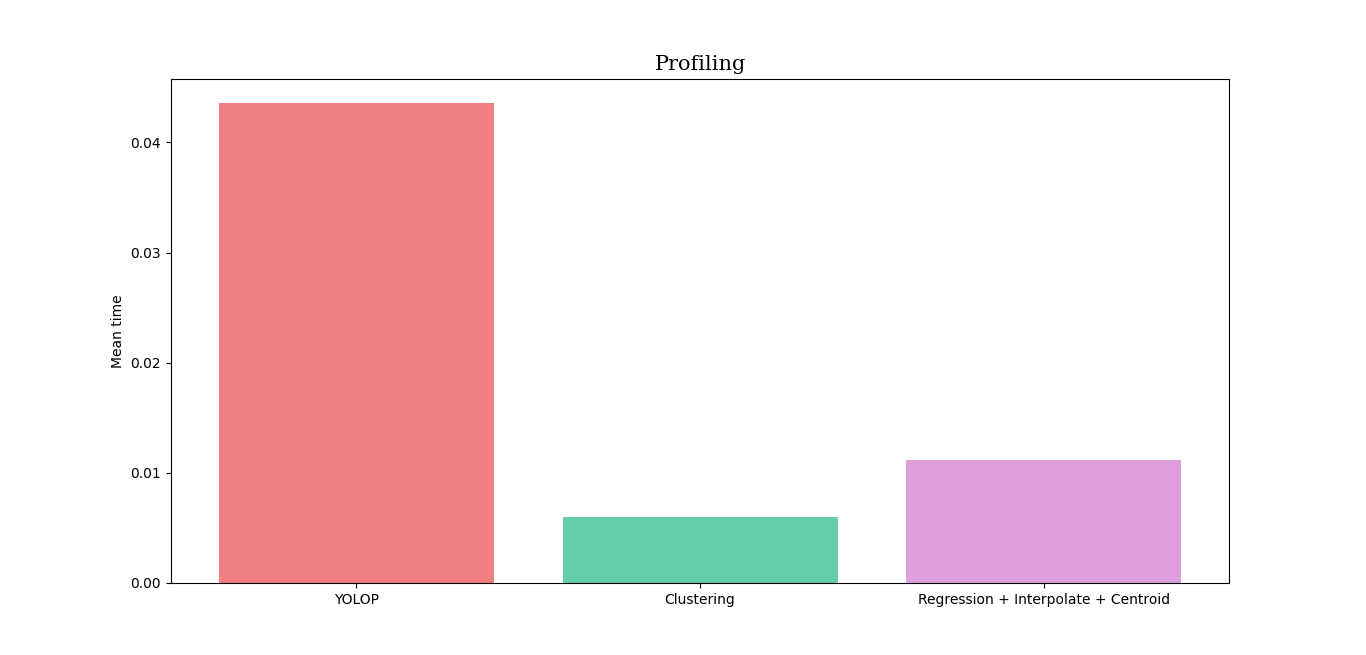
\includegraphics[scale=0.4]{figs/Diseño/Percepcion/time_profiling.png}
    \end{center}
    \caption{Profiling de las partes de la percepción}
    \label{fig:centro de masas}
  \end{figure}\

  Como podemos apreciar, la parte de la percepción que tarda más es el cálculo de la regresiones cuadráticas, la interpolación y el cálculo del centroide. Esto se debe a que
  cuando se realiza el cálculo de las regresiones hay que recorrer los puntos de los grupos de clústeres y cálcular sus funciones para obtener las regresiones. Respecto al 
  tiempo que tarda el algoritmo de DBSCAN junto con la clasficación de los clústeres es el ganador en cuanto menor tiempo de cómputo lo cual es interesante trabajar 
  con dicho algoritmo de clustering. En conclusión, sumando todos los tiempos de cada parte obtenemos un tiempo global de 0.033 segundos pasado a FPS conseguimos un rate aproximadamente
  de 30 FPS. 

  \section{Seguimiento del carril mediante control clásico}
  \label{sec:Control}

  Una vez realizado el comportamiento de la percepción, construiremos un comportamiento autónomo con el dron basandonos en un simple controlador PID. 
 Con este primer comportamiento queremos demostrar la funcionalidad de la percepción utilizando un controlador de movimiento sencillo. \newline

 Un controlador PID (proporcional, derivativo e integral) es un 
  es un sistema que es capaz de mantener una variable (como la temperatura, velocidad o posición) cercana a un valor deseado o de referencia. Cada componente de un controlador tiene un papel 
  importante,
  la componente P (proporcional) ajusta la salida del controlador en función de la diferencia entre el valor medido y el valor deseado. 
  Cuanto mayor sea esta diferencia (error), mayor será la corrección aplicada. Sin embargo, el control proporcional solo no puede eliminar completamente el error por ello se utiliza
  las componentes derivativa e integral. La componente D (derivativa) considera la tasa de cambio del error,
  si el error cambia rápidamente, el término derivativo aplicará una corrección para evitar oscilaciones o inestabilidad.
  Con el término integral se acumula el error a lo largo del tiempo y ajusta la salida del controlador en función de esta acumulación. 
  Ayuda a eliminar el error persistente o constante. Si el error es pequeño pero persistente, el término integral lo corregirá gradualmente.
  \newline

  Lo cual con este controlador PID sencillo se controlan las velocidades respecto al error que se produce entre posición deseada y la que obtenemos. La variable deseada para estar alineados con el carril se escoge
  el eje de las x el valor central de la imagen, ya que queremos en todo momento permanecer centrales respecto al carril. Para calcular el error se calcula la diferencia del valor deseado que seria 
  el valor central de la imagen y el valor del centroide del carril mencionado en la sección \ref{sec:Interpolación y cálculo del centro de masas del carril}. 
  A parte de este controlador, se utiliza un pequeño controlador PD para controlar la altura del vehículo y tengamos una altura medianamente constante. Para saber a qué altitud nos encontramos se utiliza el sensor del Lidar.

  Para encontrar los valores de cada término que compone ambos controladores se ha realizado a base de experimentación, empezando de manera creciente, es decir, primero utilizariamos
  la componente proporcional para ver su comportamiento, una vez que tengamos el valor del término proporcional pasaremos al término derivativo para suavizar los movimientos que puede
  producir este término y por último utilizariamos la parte integral para eliminar el error. El controlador PID se usará para controlar la velocidad de giro del dron en cuanto a la velocidad lineal 
  tendremos un valor constante. En el código \ref{cod:ValoresPID} se expone los valores de cada componente en ambos controladores.\newline

  \begin{code}[h]
    \begin{lstlisting}[language=Python]

      kp_height = 0.1
      kd_height = 0.4

      kp_speed_controller = 0.09
      kd_speed_controller = 0.1
      ki_speed_controller = 0.008
     
    \end{lstlisting}
    \caption[Valores de las variables del PD del control de altura y del PID del controlador de velocidad angular]{Valores de las variables del PD del control de altura y del PID del controlador de velocidad angular}
    \label{cod:ValoresPID}
    \end{code} 

  \section{Seguimiento del carril mediante aprendizaje por refuerzo}
  \label{sec:aprendizaje por refuerzo}

  Como mencionamos en la sección \ref{sec:IA},el aprendizaje por refuerzo consiste en enseñar un agente 
  desempeñar un comportamiento mediante recompensas y penalizaciones. Este comportamiento se aprende a base de interacciones con el entorno de trabajo y observaciones de como puede responder,
  de forma similar a los niños que exploran el mundo que les rodea y aprenden las acciones que les ayudan a alcanzar un objetivo. Se compone de diferentes elementos claves que se definen
  al problema a resolver del seguimiento del carril:
  \begin{itemize} 
    \item \textbf{Agente}: El agente es una entidad o modelo que pretendemos entrenar para que aprenda a tomar decisiones (acciones) en función del estado en el que nos encontremos. Nuestro 
    agente se trata del dron.
    \item \textbf{Entorno}: Ambiente en donde interactua el agente para que pueda aprendar el comportamiento deseado. El dron estará interectuando sobre el entorno de Coastline que nos proporciona Airsim 
    durante las fases de pruebas. 
    \begin{figure} [H]
      \begin{center}
        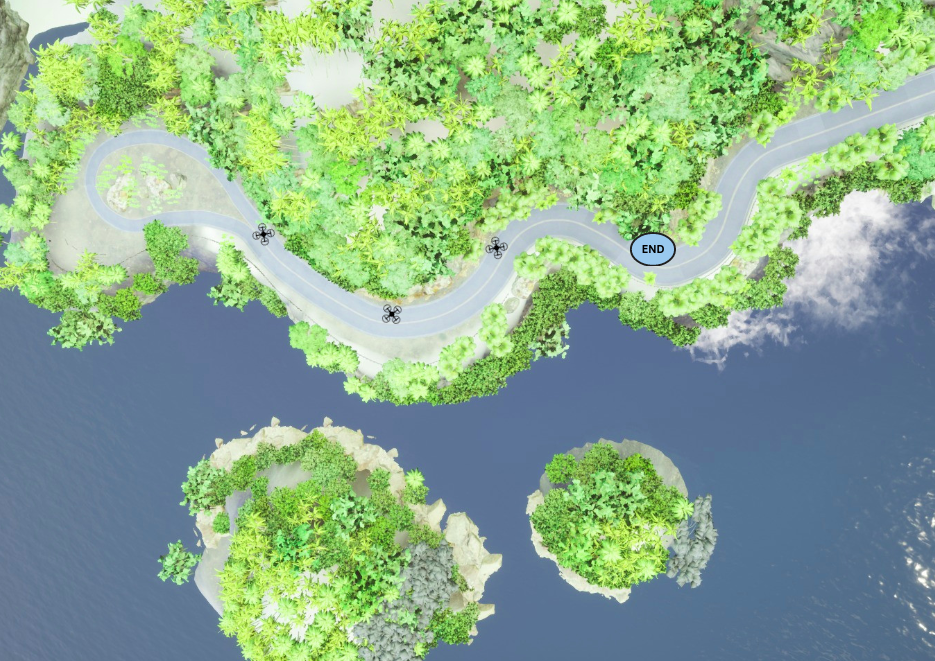
\includegraphics[scale=0.4]{figs/Diseño/RL/entorno.png}
      \end{center}
      \caption{Entorno en la fase de entrenamiento del sigue carril basado en Q-Leaning}
      \label{fig:Entorno}
    \end{figure}\

    Dentro de este circuito, hemos escogido tres localizaciones distintas para el vehículo a la hora de realizar el entrenamiento con el algoritmo de Q-Learning y el punto final del recorrido. Como se puede apreciar en la figura \ref{fig:Entorno} las posiciones
    tienen una distancia entre ellas considerablemente. 
    \item \textbf{Estados}: Condiciones en las que se puede encontrar el agente en ese instante de tiempo. Para la definición de los estados, se divide la imagen que damos como la salida de la detección del carril en 14 franjas, dichas franjas tienen una 
    separación de 10 pixeles. Las franjas representan cada estado en el que se puede encontrar el agente. Empezamos a definir el primer estado desde la izquierda hasta la derecha con una
    hasta conseguir los 14 estados correspondientes, 7 estados izquierda, 1 estado central y 6 estados derecha. Se puede observar el resultado de los estados en la figura \ref{fig:Estados}

    \begin{figure} [H]
      \begin{center}
        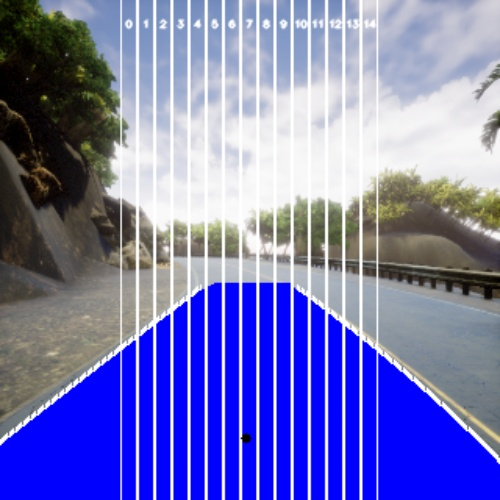
\includegraphics[scale=0.5]{figs/Diseño/RL/estados.jpg}
      \end{center}
      \caption{Estados definidos para el sigue carril basado en Q-Learning}
      \label{fig:Estados}
    \end{figure}\

    \item \textbf{Acciones}: Movimientos que puede realizar el agente dentro del estado en el entorno de entrenamiento. En total, se definen 21 acciones, que podrá escoger el agente en el algoritmo de Q-Learning. Se componen de pares de velocidades lineales y angulares, las velocidades lineales
    tendrán un intervalo de 0.1 m/s hasta 2.0 m/s. Así siendo el intervalo de la velocidad angular de -25 hasta 25 grados/segundo, teniendo giros hacia la izquierda y hacia la derecha. Dichos pares
    de velocidades serán formados a partir de la función que nos proporciona numpy llamada linspace\footnote{\url{https://numpy.org/doc/stable/reference/generated/numpy.linspace.html}}. \newline
  
    \begin{code}[H]
      \begin{lstlisting}[language=Python]
  
        
        def build_actions():
            ACTIONS = []
            speeds_actions = np.linspace(0.1,2.0,11, dtype=float)
            angular_speeds = np.linspace(-25,25, 21)
        
            left_angular_speeds = angular_speeds[:10]
            right_angular_speeds = np.flip(angular_speeds[-10:])
            central_angular_speed = angular_speeds[10]
            speeds = speeds_actions[:10]
            central_speed = speeds_actions[10]
        
            for i in range(len(speeds)):
                ACTIONS.append([round(speeds[i],3),round(left_angular_speeds[i],3)])
        
            ACTIONS.append([round(central_speed,3),0.0])
        
            for  i in reversed (range(len(speeds))):
                ACTIONS.append([round(speeds[i],3),round(right_angular_speeds[i],3)])
  
            return ACTIONS
       
      \end{lstlisting}
      \caption[Construcción de las acciones para Q-Learning]{Construcción de las acciones para Q-Learning}
      \label{cod:Acciones}
      \end{code}
      
    \item \textbf{Función de Recompensa o Penalizaciones}: Consiste en como queremos premiar o penalizar al agente con el objetivo que queremos cumplir. Las recompensas o penalizaciones se recogen
    en una función, dicha función es independiente en cada diseño del objetivo que quiere completar el agente. La función de recompensa se compone de dos partes premiando al dron de que
    permanezca centrado en el carril y además preamiarle por mantener una orientación adecuada respecto al carril, asegurando que se navegue de forma paralela al mismo. Cada parte tiene un peso
    de importancia, siendo el peso que se permanezca del carril del 85\% y la orientación respecto al carril de un 15\%. Tanto la recompensa por mantenerse centrado en el carril 
    como la orientación respecto al carril es normalizada entre valores de 0-1, penalizando con un valor constante al dron cuando se salga del carril o 
    se pierda la percepción. La implementación de la función de recompensa y las penalizaciones se puede ver en el código \ref{cod:recompensa}:

    \begin{code}[H]
      \begin{lstlisting}[language=Python]
  
        def reward_function(self,cx,angle):

        reward = 0
        target_heading = 0
        error_lane_center = (WIDTH/2 - cx)
        heading_difference = (target_heading - angle) 
        
        MIN_ERROR = 0
        MAX_ERROR = 80

        MIN_ANGLE = 0
        MAX_ANGLE = 70

        CENTRE_WEIGHT = 0.85
        ANGLE_WEIGHT = 0.15
        
        if (self.is_exit_lane(cx)):
            
            reward = -10

        else:

            
            normalise_error_centre = (abs(error_lane_center) - MIN_ERROR) / (MAX_ERROR - MIN_ERROR)
            reward_centre = 1 - normalise_error_centre

            
            normalise_error_angle = (abs(heading_difference) - MIN_ANGLE) / (MAX_ANGLE - MIN_ANGLE)
            reward_angle = 1 - normalise_error_angle


            reward = (reward_centre * CENTRE_WEIGHT) + (reward_angle * ANGLE_WEIGHT)
            
        return reward
       
      \end{lstlisting}
      \caption[Función de recompensa]{Función de recompensa}
      \label{cod:recompensa}
      \end{code}
    \item \textbf{Política}: Determina que acción realizar en cada estado que se encuentre el agente. Dicha política varía según el tipo de algoritmo que queremos seguir dentro de aprendizaje por refuerzo.
    Puede ser determinista o estocástica.

    En este TFG, se sigue una política epsilon-greedy\cite{Epsilon-greedy}, que consiste 
 equilibrar la exploración y explotación en la fase de entrenamiento. Cuando el agente tenga que escoger la acción que tomar tendra en cuenta dos enfoques:
 
 \begin{itemize}
   \item Exploración (con probabilidad $\epsilon$): El agente escogerá una acción al azar para explorar
   \item Explotación(con probabilidad $ 1 - \epsilon$): El agente escogerá la acción con el valor de la tabla Q(S,A) más alto, es decir, la mejor acción conocida
 \end{itemize}
 
 El parámetro $\epsilon$ es el responsable de controlar la proporción de exploración frente a explotación, si $\epsilon$ es alto el agente explorará más en cambio si $\epsilon$ es bajo
 el agente se centrará en la explotación. Por lo que en la elección de acción se generará un numero n aleatoriamente, si n es menor que la probabilidad $\epsilon$ la acción se escogerá aleatoriamente
 en cambio si n es mayor que la probabilidad de $\epsilon$ la acción será que mayor valor tenga en la tabla Q(S,A) para dicho estado. \newline
 
 Dentro de esta política la probabilidad de $\epsilon$ será decayente, es decir, no tener un valor constante en cada episodio que nos encontremos, lo que realizaremos es una disminuición 
 de esta probabilidad para conseguir que el agente con el paso del tiempo poco a poco explote lo que ha aprendido y que el modelo llegue a una convergencia óptima. Para llevar a cabo el descenso
 de $\epsilon$ se puede realizar de varias formas, por ejemplo podemos realizarlo linealmente, logaritmicamente, exponencial o escalonado. \newline
  \end{itemize}

  El algoritmo Q-Learning se basa en seguir una función acción-recompensa formada por un tabla estado-acción la cual iremos rellenando siguiendo la siguiente ecuación
  de Bellman\cite{Bellman}:
  
  \begin{equation}
    Q(s, a) = Q(s, a) + \alpha \cdot [R(s, a) + \gamma \cdot \max Q(s', a') - Q(s, a)]
  \end{equation}

  en donde, 

  \begin{itemize}
    \item \textbf{$Q(s, a)$}: Valor Q para el estado $s$ y la acción $a$. Se trata de una matriz formada por estado y acción.
    \item \textbf{$\alpha$}: Tasa de aprendizaje entre un valor de 0 a 1. Consiste en el porcentaje que daremos al agente para el proceso de aprendizaje, 
    si dicho valor es alto daremos más peso al valor aprendido. Dicho valor se define con un valor de 0.5 
    \item \textbf{$R(s, a)$}: Recompensa por tomar la acción $a$ en el estado $s$. La función de recompensa es crucial en el proceso de aprendizaje del agente, evalua como es favorable o deseable
    es una acción tomada por el agente en el estado que se encuentre. Proporciona información al agente sobre que acciones maximizan la recompensa total a lo largo del tiempo. Dicha función
    de recompensa es diseñada dependiendo de cual sea el objetivo de tu agente. 
    \item \textbf{$\gamma$}: Factor de descuento entre un valor de 0 a 1. Modela la importancia de las recompensas futuras en relación con las recompensas inmediatas, refleja la importancia del agente
    por las recompensas a largo plazo. Un valor alto sifnigicará que le agente valorará mucho las recompensas futuras, mientras que un valor bajo indica que se enfocará más en las recompensas
    inmediatas. Dicho valor se define con un valor de 0.7.
    \item \textbf{$\max Q(s', a')$}: Valor Q máximo en el próximo estado $s'$ para todas las acciones posibles $a'$.
\end{itemize}

A la medida que vayamos avanzando en la fase de entrenamiento, iremos rellenando la tabla Q(s,a) para más adelante indexar en ella en la fase de inferencia.

\subsubsection{Fase de entrenamiento}
\label{sec:fases_ql}
 Antes de adentrarnos en esta fase, definiremos dos conceptos importantes:
 \begin{itemize}
  \item \textbf{Episodios}: Se define episodio como una secuencia completa de interacciones que se produce entre el agente y el entorno. Cada episodio comienza con un estado inicial y consta de una serie 
  de pasos o acciones tomadas por el agente.
  \item \textbf{Iteraciones (steps)}: Son los pasos que puede dar un agente en el entorno dentro de un episodio. Estos pasos pueden incluir observaciones del entorno, decisiones tomadas por el agente
  y las consecuentes recompensas o penalizaciones recibidas.
\end{itemize}

 
 La fase de entrenamiento consiste en el que el agente explore todo lo máximo posible en el entorno respecto a los estados que tiene y las acciones que puede tomar, es decir, al comienzo del entrenamiento se inicializará la tabla Q(S,A) a cero todos sus valores, esta representación
 al comienzo es así ya que el agente desconoce por completo el entorno hasta que poco a poco vaya iterando sobre él en cada estado tomando x accion. \newline
 
 Basicamente, en cada iteración del algoritmo se escogerá una acción según si estamos en exploración o explotación, se calculará la recompensa obtenida e iteraremos de nuevo sobre el algoritmo.

 El entrenamiento finaliza cuando el agente haya aprendido el objetivo que queremos seguir, esto se sabe cuando las iteraciones del algoritmo y la recompensa acumulada del agente en esta 
 fase se estabilice y tenga valores constantes, es decir, no cambia significativamente con más iteraciones, esto se denomina que el modelo ha convergido y pasaremos a la fase de inferencia. \newline

Durante esta fase, dejamos el algoritmo de Q-Learning entrenando durante aproximadamente 12 horas teniendo un rate del algoritmo de Q-Learning más el algoritmo de percepción aproximadamente de 
unos 10 FPS. De esta manera, nos podemos asegurar que el algoritmo completará el entrenamiento de manera correcta y poco a poco 
acabará convergiendo. 
En la figura \ref{fig:entrenamiento} se ilustra la fase de entrenamiento durante la navegación del dron. En la primera figura se corresponde al número de iteraciones de cada 
episodio durante el entrenamiento, la segunda corresponde al valor que va teniendo épsilon en cada episodio y la tercera grafica se muestra el valor de la recompensa 
acumulativa en cada episodio. \newline

\begin{figure} [H]
  \begin{center}
    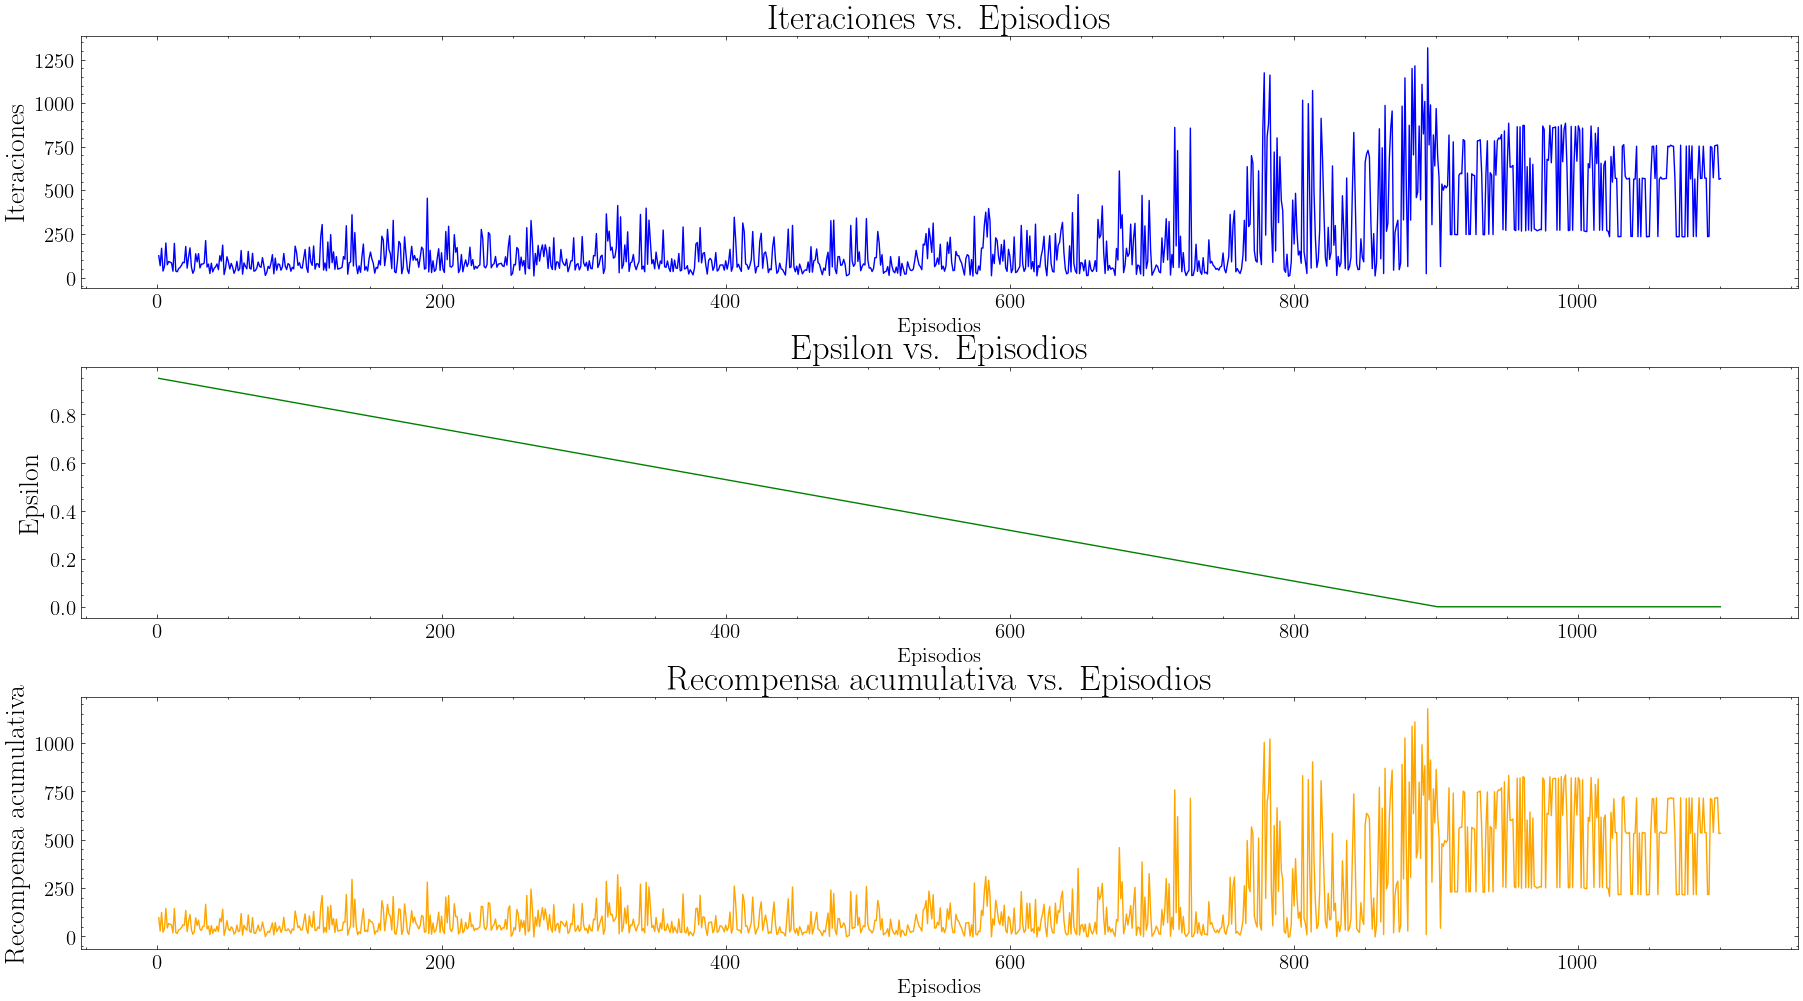
\includegraphics[scale=0.35]{figs/Diseño/RL/graficas-entrenamiento.png}
  \end{center}
  \caption{Gráficas de la fase de entrenamiento}
  \label{fig:entrenamiento}
\end{figure}\

Al comienzo del entrenamiento, se puede observar que el dron obtiene pocas iteraciones y bajas recompensas acumulativas, 
esto se debe a que el dron al comienzo del entrenamiento desconoce por completo el entorno. A medida que vamos avanzando en el entrenamiento, 
las iteraciones y los valores de la recompensa acumulativa son mayores hasta que en el episodio 900 donde acaba la fase de exploración 
siendo el valor de épsilon cero (las acciones no son aleatorias). A partir de ese punto, la recompensa y las iteraciones tienen una tendencia ascendente, y finalmente, 
a lo largo del entrenamiento, ambas se estabilizan en un valor fijo sin cambiar considerablemente. Esto se debe a que el dron completa constantemente el circuito en cualquier
punto de reinicio dentro del circuito mostrado en la figura \ref{fig:Entorno} sin cambiar considerablemente la tabla Q. En este momento, se puede decir que el algoritmo ha sido capaz de converger. Una vez se analice 
los resultados del entrenamiento con las diferentes métricas daremos pie a la fase de inferencia para verificar el resultado obtenido con el modelo entrenado. 

\subsubsection{Fase de inferencia}
\label{sec:fases_inferencia}
La fase de inferencia consiste en indexar la tabla Q(S,A) que hemos ido rellenando en la fase de entrenamiento. El dron cuando se encuentré en un estado especifico consultará la tabla Q(S,A) para
encontrar la mejor acción en ese estado (cuando mencionamos la mejor acción nos referimos al máximo valor en la tabla que tenga en ese estado). Cuando el dron tome dicha acción se moverá al siguiente estado
siendo así un proceso iterativo hasta alcanzar la meta. En esta fase, los valores de la tabla permanecen constantes y se utiliza para la toma de decisiones basadas en el conocimiento
aprendido en la fase de entrenamiento. \newline

En la figura \ref{fig:Distribucción_inferencia} se puede observar las diferentes acciones que ha utilizado el dron para completar el circuito de entrenamiento utilizando cuatro de veintiuno de acciones
disponibles. Se destaca que la acción más usada se trata de una de las acciones que presentan poco giro y alta velocidad lineal dentro de las acciones con más velocidad lineal, esto se debe
a la importancia de la función de recompensa al considerar que queremos que el dron se mantenga constantemente en el centro del carril manteniendo un angulo de orientación adecuado
sin salirse del carril.

\begin{figure} [H]
  \begin{center}
    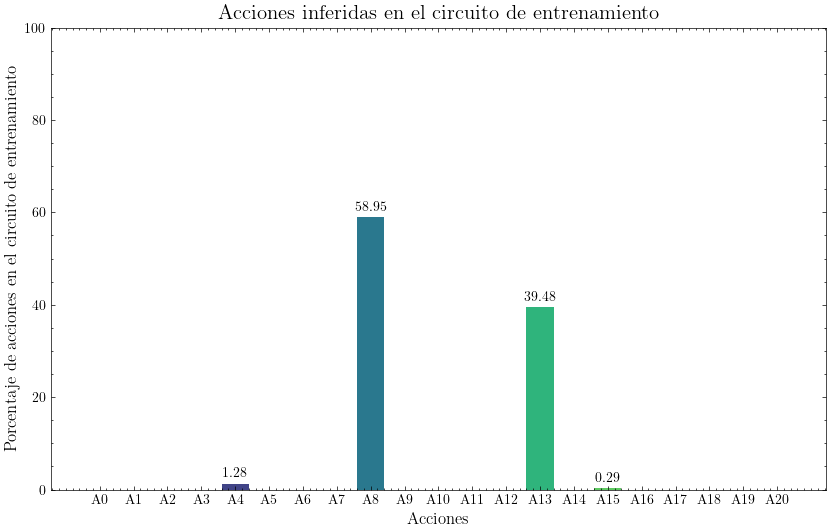
\includegraphics[scale=0.7]{figs/Diseño/RL/Acciones_inferidas.png}
  \end{center}
  \caption{Distribucción de acciones en el circuito de entrenamiento}
  \label{fig:Distribucción_inferencia}
\end{figure}\

Como resultado al utilizar el algoritmo de Q-learning, el modelo entrenado ofreció ser un resultado eficaz a la hora de navegar por el circuito, pudiendo observar 
el modelo entrenado final en diferentes localizaciones alteatorias en el entorno de la figura \ref{fig:Entorno}. Para poder obtener el máximo rendimiento del modelo entrenado se busco los límites de velocidad
angular y lineal a la que podía ir el dron, esto significa multiplicar por un factor todas las acciones tanto las velocidades lineales y angulares. Este proceso es interesante 
realizarlo para maximizar el comportamiento sin la necesidad de volver a entrenar un nuevo modelo. Estos factores se pueden ver en el código \ref{cod:Factores} lo cual 
las acciones se pueden aumentar un 100\% lo que podemos decir que el modelo entrenado es efectivo al aumentar el valor de las acciones. \newline

\begin{code}[h]
  \begin{lstlisting}[language=Python]

    factor_speed = 2.0
    factor_angular_speed = 1.8
   
  \end{lstlisting}
  \caption[Factores]{Valores de los factores aplicados a las acciones de Q-learning}
  \label{cod:Factores}
  \end{code} 

Siendo los nuevos valores de las acciones utilizados durante las fases de comparación entre el seguimiento de carril con el PID y el seguimiento de carril mediante Q-Learning. Los nuevos
valores de las acciones originales como se mostraba en el código \ref{cod:Acciones} son multiplicados por ambos factores
y su gráfico de acciones como se muestra en la figura \ref{fig:inferencia_factor}. Se puede observar que en la distribución de acciones el dron
sigue escogiendo acciones con velocidad lineal alta y velocidad angular baja para mantenerse dentro del recorrido sin salirse, además de aumentar el porcentaje de las acciones escogidas respecto a la distribución de acciones
que se mostraba en la figura \ref{fig:Distribucción_inferencia}

\begin{figure} [H]
  \begin{center}
    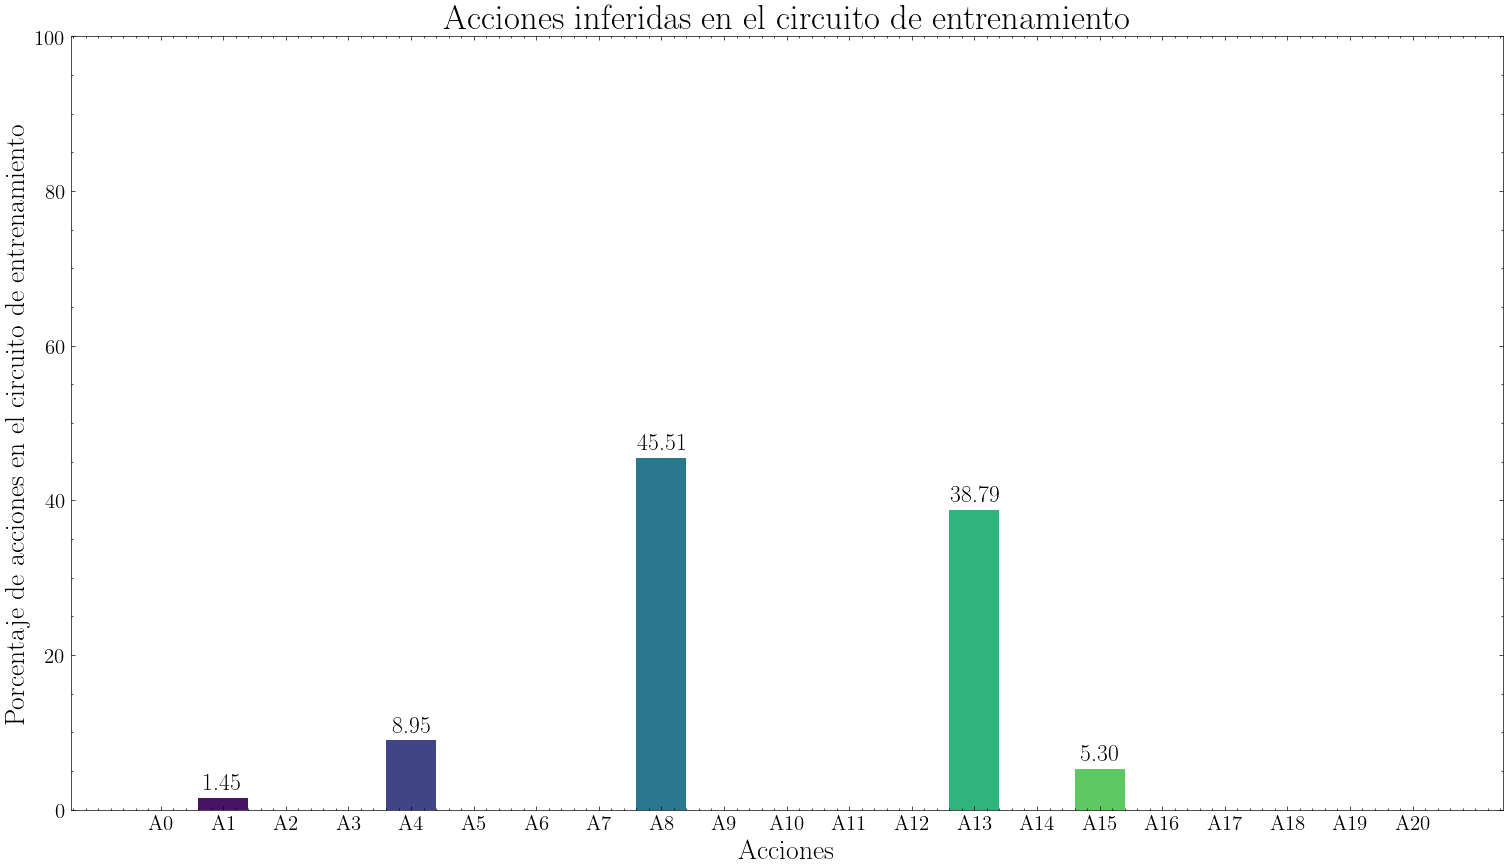
\includegraphics[scale=0.4]{figs/Diseño/RL/Acciones_inferidas_factor.png}
  \end{center}
  \caption{Distribucción de acciones en el circuito de entrenamiento multiplicadas por el factor}
  \label{fig:inferencia_factor}
\end{figure}\


\subsection{Análisis y comparativa entre el seguiento de carril clásico}
\label{sec:Análisis y comparativa entre el seguiento de carril clásico}
Para comprobar la robustez y la eficacia que demuestra ser el modelo entrenado junto con el seguimiento de carril mediante el PID, se realizo varias comparativas en ambos
comportamientos. Se ajusto las velocidades del controlador PID para que ambos tuviesen las mismas condiciones, para ello se utilizo un circuito en el que ambos son capaces 
de recorrerlo sin salirse del carril. En la figura \ref{fig:comparativa} se muestra el resultado de ambos comportamientos, en la primera figura es todo el recorrido hasta el punto
final y en la segunda figura se realiza zoom en una parte del recorrido, los datos fueron recogidos mediante la posición del dron guardandolos un fichero tanto las coordenadas 
en el eje x como las coordenadas en el eje y. 
  
\begin{figure}[H]
  \centering
  \begin{minipage}{1.0\textwidth}
    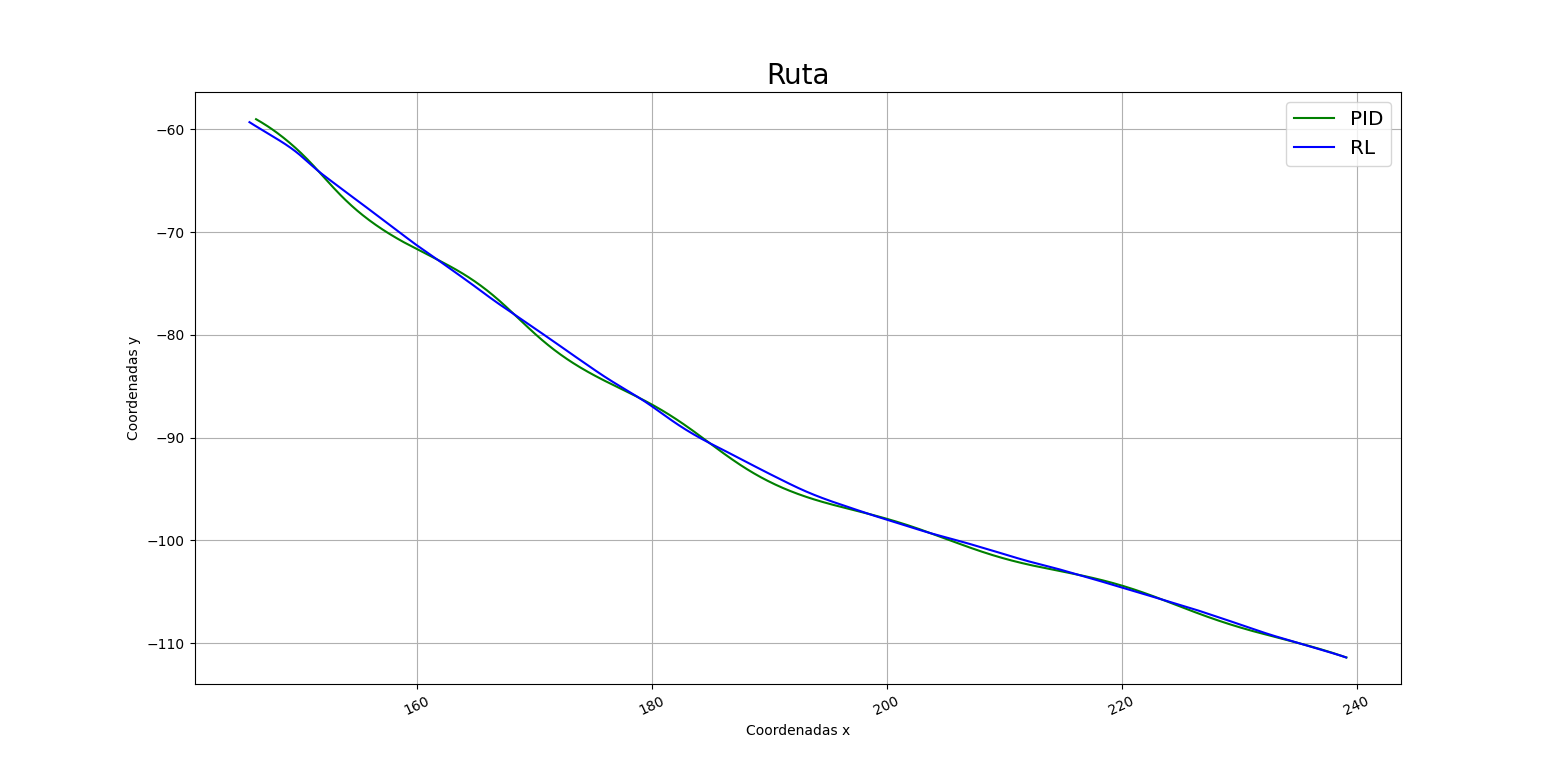
\includegraphics[width=\linewidth]{figs/Diseño/RL/ruta.png}
  \end{minipage}
  \hfill
  \begin{minipage}{1.0\textwidth}
    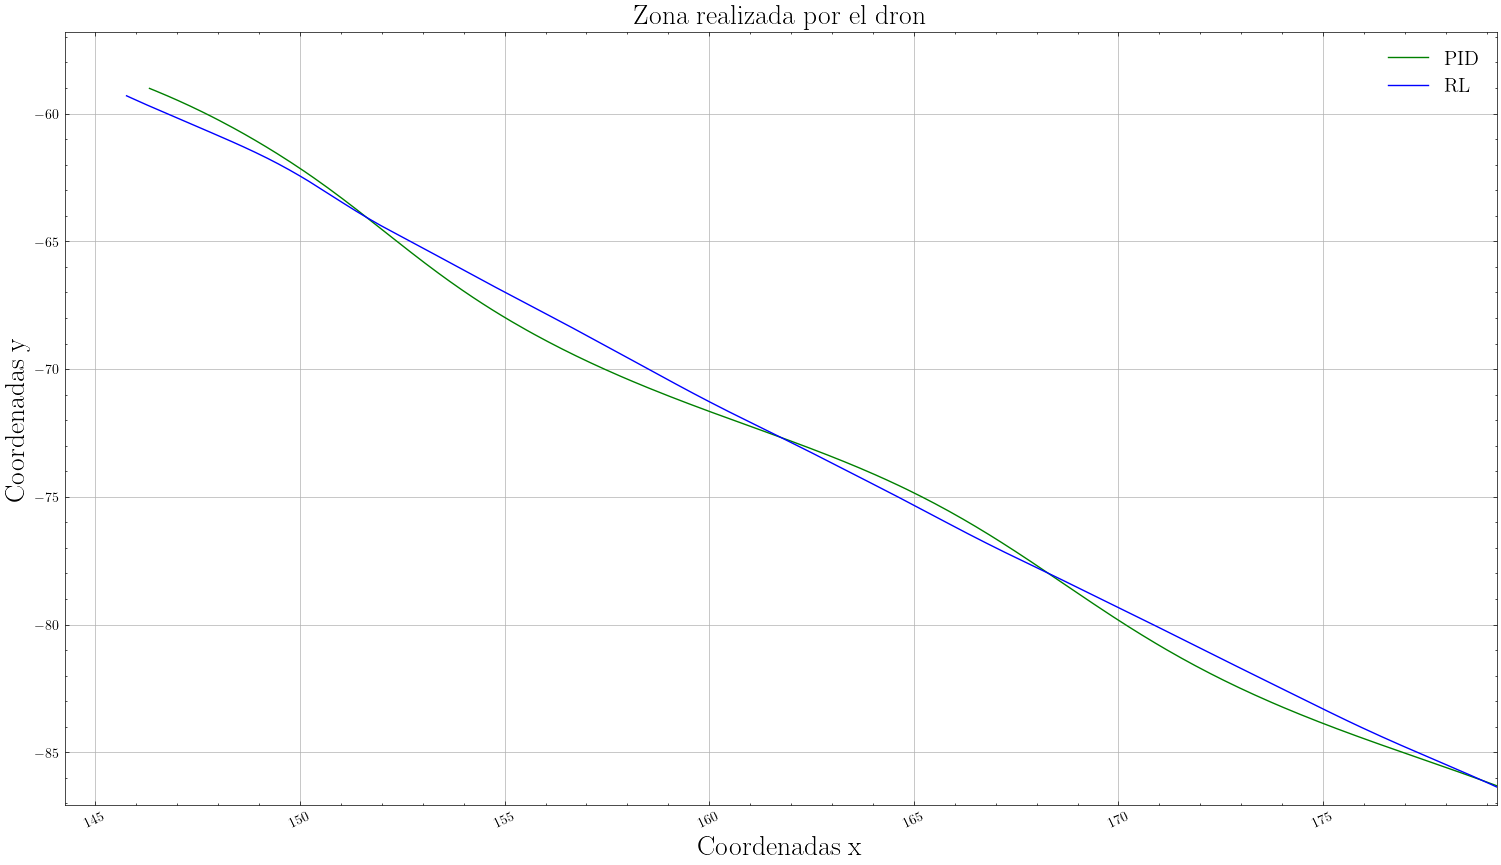
\includegraphics[width=\linewidth]{figs/Diseño/RL/ruta_zoom.png}
  \end{minipage}
  \caption{Comparativa realizando un trayecto entre ambos comportamientos}
  \label{fig:comparativa}
\end{figure}

Una de las principales diferencias entre ambos comportamientos es que el comportamiento con control clásico presenta oscilaciones durante el recorrido relizando eses 
por ambas partes del recorrido hasta llegar al punto final del recorrido. En cambio, el comportamiento con aprendizaje por refuerzo destaca por su trayectoria constante 
durante todo el recorrido sin apenas realizar oscilaciones, destacando que el trayecto para realizar la comparativa se trata de un trayecto recto sin apenas curvas que se 
puede visualizar en la figura \ref{fig:trayectoPID}.

\begin{figure} [H]
  \begin{center}
    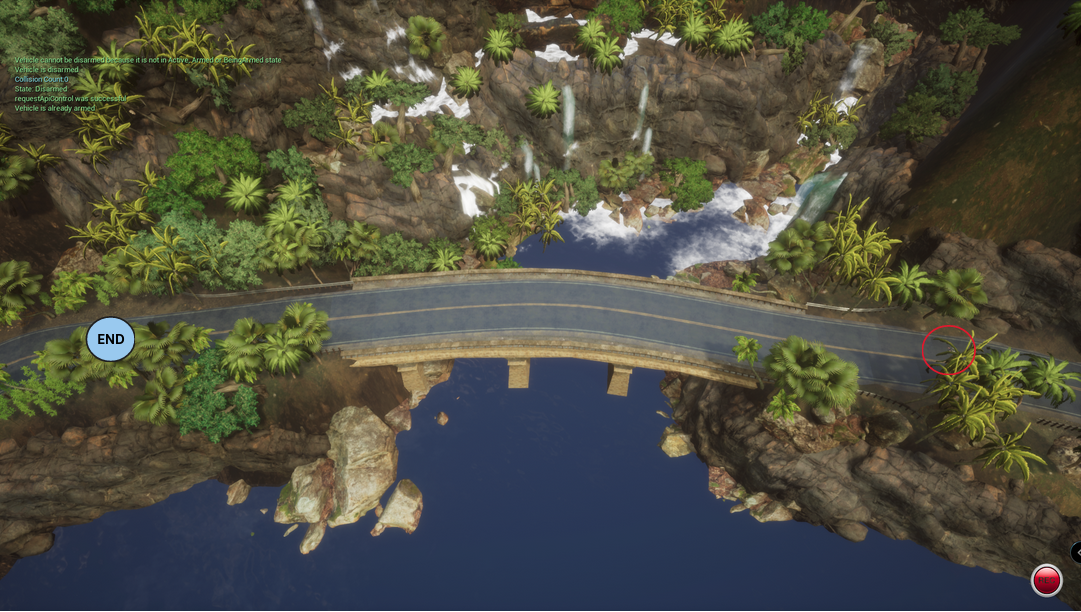
\includegraphics[scale=0.4]{figs/Diseño/RL/trayecto1.png}
  \end{center}
  \caption{Trayecto en donde se realiza la comparativa entre el PID y aprendizaje por refuerzo}
  \label{fig:trayectoPID}
\end{figure}\

Finalmente, en la figura \ref{fig:media_velocidades} se ilustra la media de velocidades angulares que han obtenido ambos comportamientos en el recorrido. Dichas velocidades
se han ido almacenando a la medida que el dron recorría el trayecto. Se puede apreciar como el comportamiento de aprendizaje por refuerzo obtiene menor media de velocidad angular respecto al controlador PID manteniendo un trayectoria segura y eficaz en un recorrido 
que nunca ha visto durante la fase de entrenamiento sin realizar apenas oscilaciones durante todo el trayecto. Respecto, al controlador PID, mantiene una media angular alta debido a que 
necesita realizar ajustes para mantenerse en el trayecto constantemente resultando tener una mayor giro para permanecer central al carril. \newline
En este tipo de trayectos, el comportamiento de aprendizaje por refuerzo demuestra ser más eficiente que el controlador PID sin requerir muchos ajustes respecto a la velocidad
angular para manterse en la trayectoria y es capaz de adaptarse a cualquier recorrido del entorno.

\begin{figure} [H]
  \begin{center}
    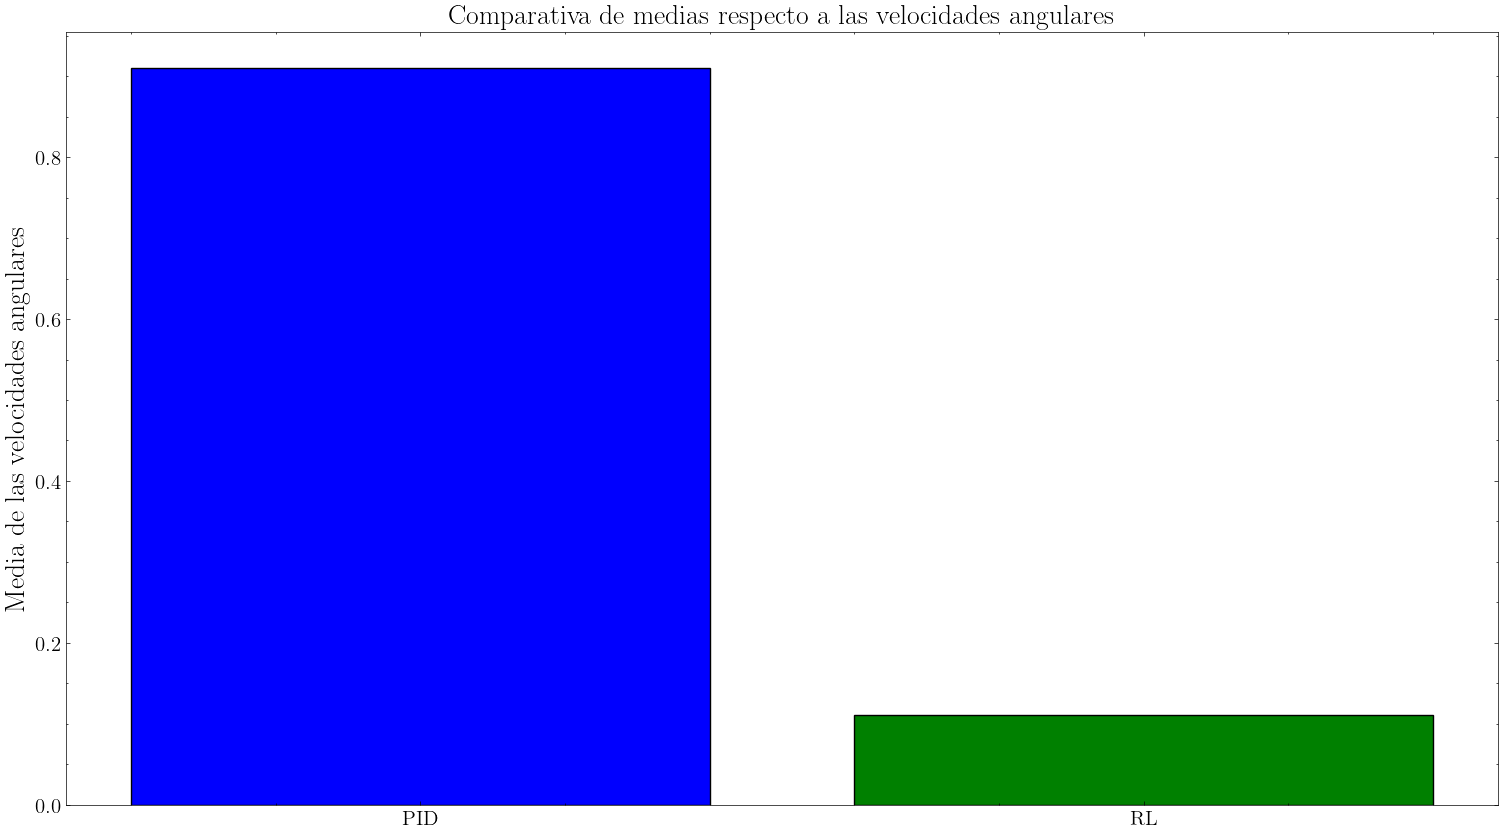
\includegraphics[scale=0.4]{figs/Diseño/RL/medias_velocidades_angulares.png}
  \end{center}
  \caption{Media de velocidades angulares de ambos comportamientos desarrollados}
  \label{fig:media_velocidades}
\end{figure}\

Demostrando asi que el modelo entrenado es capaz de obtener comportamientos satisfactorios tomando acciones acordes
al recorrido de entrenamento u recorridos que no ha visto durante en la fase de entrenamiento. En la figura \ref{fig:comparativa}, se muestra diferentes frames 
durante el recorrido siendo capaz de manternerse centrado al carril. 

\begin{figure}[H]
  \centering
  \begin{minipage}{0.3\textwidth}
    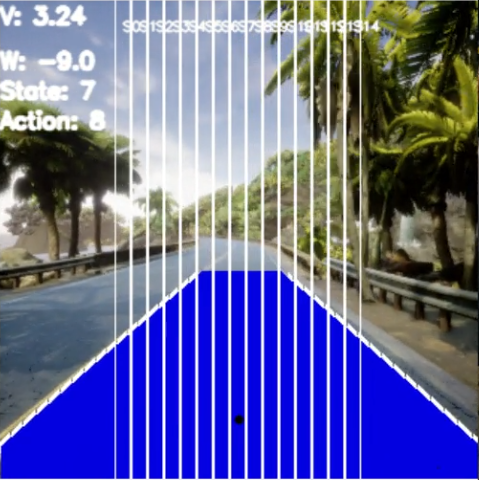
\includegraphics[width=\linewidth]{figs/Diseño/RL/rl1.png}
  \end{minipage}
  \hfill
  \begin{minipage}{0.3\textwidth}
    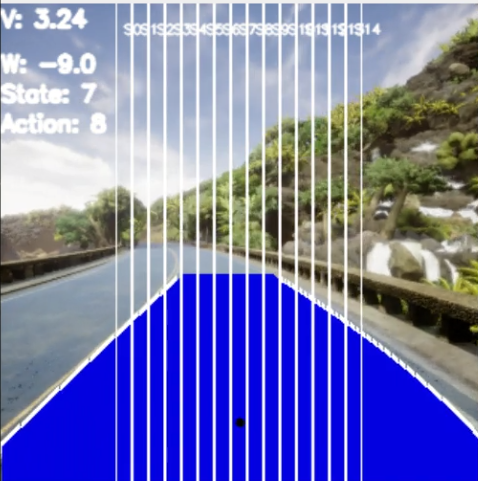
\includegraphics[width=\linewidth]{figs/Diseño/RL/rl2.png}
  \end{minipage}
  \hfill
  \begin{minipage}{0.3\textwidth}
    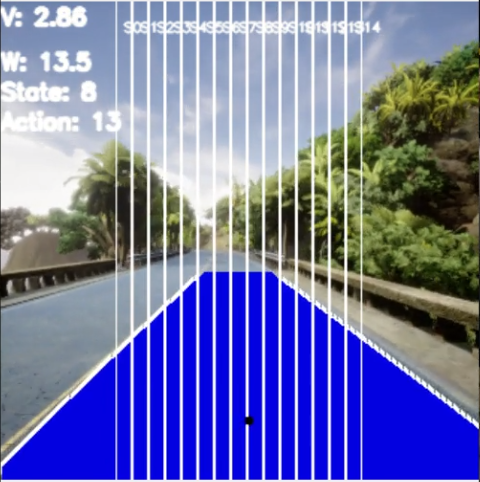
\includegraphics[width=\linewidth]{figs/Diseño/RL/rl3.png}
  \end{minipage}
  \caption{Resultado del comportamiento de aprendizaje por refuerzo ilustrando los estados y acciones teniendo en cuenta el factor}
  \label{fig:comparativa}
\end{figure}














        


  

